\documentclass{article}

% if you need to pass options to natbib, use, e.g.:
%     \PassOptionsToPackage{numbers, compress}{natbib}
% before loading aaj2026


% ready for submission
\usepackage[final]{aaj2026}
\bibliographystyle{IEEEtran}
% use CJKutf8 for Chinese characters
\usepackage{ctex}

% to compile a preprint version, e.g., for submission to arXiv, add add the
% [preprint] option:
%     \usepackage[preprint]{aaj2026}


% to compile a camera-ready version, add the [final] option, e.g.:
%     \usepackage[final]{aaj2026}


% to avoid loading the natbib package, add option nonatbib:
%    \usepackage[nonatbib]{aaj2026}


\usepackage[utf8]{inputenc} % allow utf-8 input
\usepackage[T1]{fontenc}    % use 8-bit T1 fonts
\usepackage{hyperref}       % hyperlinks
\usepackage{url}            % simple URL typesetting
\usepackage{booktabs}       % professional-quality tables
\usepackage{amsfonts}       % blackboard math symbols
\usepackage{nicefrac}       % compact symbols for 1/2, etc.
\usepackage{microtype}      % microtypography
\usepackage[table]{xcolor}         % colors
\usepackage[most]{tcolorbox} % colored boxes
\usepackage{graphicx}       % graphics
\usepackage{tikz}
\usepackage{caption}
\usepackage{makecell}
\definecolor{coverlinecolor}{HTML}{002FA7}
\newcommand{\foo}{\color{coverlinecolor}\makebox[0pt]{\textbullet}\hskip-0.5pt\vrule width 1pt\hspace{\labelsep}}
\usetikzlibrary{arrows.meta, positioning, shapes.geometric, calc}

\title{Topological Feature Analysis of focus music Based on Path Homology and Its Application in ACE-Step Latent Space Guided Generation}


% The \author macro works with any number of authors. There are two commands
% used to separate the names and addresses of multiple authors: \And and \AND.
%
% Using \And between authors leaves it to LaTeX to determine where to break the
% lines. Using \AND forces a line break at that point. So, if LaTeX puts 3 of 4
% authors names on the first line, and the last on the second line, try using
% \AND instead of \And before the third author name.


\author{%
  Fisher E. Yu \\
  \texttt{September 12, 2026} \\
}


% 信息页关闭页面锚点，避免与正文第 1 页的页码重复
\hypersetup{pageanchor=false}

\begin{document}

% ======== 参赛信息页（不计入正文页码）========
\thispagestyle{empty}
\begin{center}
  \vspace*{3cm}
%   {\zihao{2}\heiti 参赛信息页\par}
%   \vspace{2cm}
  \renewcommand{\arraystretch}{2.2}
  {\zihao{3}
  \begin{tabular}{r@{：}l}
    参赛学生姓名 & \underline{\makebox[9cm][l]{于儿 \; Fisher E. Yu}} \\
    中学         & \underline{\makebox[9cm][l]{华南师范大学附属中学}} \\
    省份         & \underline{\makebox[9cm][l]{广东省}} \\
    国家/地区    & \underline{\makebox[9cm][l]{中国}} \\
    指导老师姓名 & \underline{\makebox[9cm][l]{杨晓安，肖天昂}} \\
    指导老师单位 & \underline{\makebox[9cm][l]{华南师范大学附属中学，谱蓝云}} \\
    论文题目     & \parbox[t]{9cm}{%
        \linespread{1.5}\selectfont
      \underline{\makebox[9cm][l]{Topological Feature Analysis of Focus}}\\
      \underline{\makebox[9cm][l]{Music Based on Path Homology and Its}}\\
      \underline{\makebox[9cm][l]{Application in ACE-Step Latent Space}}\\
      \underline{\makebox[9cm][l]{Guided Generation}}%
    } \\
  \end{tabular}}
\end{center}
\clearpage
\setcounter{page}{1}
\hypersetup{pageanchor=true}
% ======== 参赛信息页结束 =====

\maketitle


\begin{abstract}
  功能性专注音乐被广泛用于学习与工作场景，但其区别于一般音乐的时序结构仍缺少可计算、可审计且可用于生成控制的表示。本文将音乐建模为随时间演化的有向动态系统，在由 $300$ 首 Open Focus 与 $300$ 首 Classical 器乐组成、具有逐曲来源与许可记录的数据集上，采用``发现拟合---冻结---主要验证---时长敏感性''流程，结合 GLMY 路径同调与相位提升路径同调，比较局部状态转移和跨周期相位闭合。validation/180s 的主要分析表明：音高与节奏视角分别有 $13/20$ 和 $14/20$ 个预设指标通过 BH-FDR；Classical 通常具有更广的状态覆盖与转移多样性，而 Open Focus 具有更高的自转移比例和有向复现率。调制视角有 $5/20$ 个指标通过主分析 FDR，但因其 SMP-$K=10$ 表征是在 holdout 开启后提出，仅作探索性解释。三个局部视角均未获得稳定的 $H_1$ 组间差异。宏观尺度上，Open Focus 的 Acoustic 与 Chroma 相位 \texttt{loop\_score} 高于 Classical，rank-biserial 效应量分别为 $0.459$ 与 $0.338$，且通过三视角 BH-FDR；Rhythm phase 在主要尺度未通过 FDR。多尺度分析显示，Pitch、Phase 及其联合空间均存在组间距离差异，但联合表示并未优于最佳单块。基于上述结果，本文为后续未见数据与生成实验冻结由 $16$ 维 Pitch、Acoustic phase 与 Chroma phase 各一维组成的 $18$ 维指纹，平方距离权重为 $1/2:1/4:1/4$。进一步地，本文在 ACE-Step 1.5 上实现了``精确 Path Homology 教师---可微潜空间代理---精确复核''推理期引导协议：以逐采样步预测干净潜变量的精确拓扑标签训练代理网络，在未见 prompt、seed family 与生成轨迹上完成并通过坐标预测、候选排序、不确定度校准及 OOD/no-op 资格检验，随后以 $512$ 首 baseline/guided 配对音频完成最终评价。该评价以冻结精确拓扑目标带为主要终点，并将 prompt 一致性、音质、多样性、运行时间与显存开销纳入预设非劣性判据，从而形成从观察性结构发现、指纹冻结到门控生成评价的完整证据链。本文结论仅涉及当前语料与冻结协议下的拓扑结构表征和生成控制，不作注意力改善或临床疗效的因果推断。
\end{abstract}


\begin{keywords}
  focus music, Topological Music Analysis, Path Homology, Persistent Path Homology, Topology-Guided Music Generation, Latent Topology Surrogate Network, ACE-Step
\end{keywords}

\clearpage

\setcounter{tocdepth}{2}
\tableofcontents

\clearpage

\section{Introduction}

% 研究背景

注意缺陷多动障碍（Attention Deficit Hyperactivity Disorder, ADHD）是一类常见的神经发育障碍，全球儿童患病率约为 $7-10\%$，成人患病率约为 $2-5\%$\cite{Siva2025}。保守估计，全球大约有 2.4 亿人不同程度地受到注意力缺失的影响。在学习、写作、编程和深度工作场景中，专注音乐常被用于支持持续注意力。有研究表明，有针对性设计的 focus music 在辅助提升注意力方面展现出了卓越的潜力 \cite{MADJAR2020113207, Phoebe2025, Erarslan2026}。

近几年，随着 EEG、fMRI 和大语言模型技术的发展，越来越多的研究开始关注功能性音乐的声学调制、统计特征与注意场景之间的关系。例如，Kevin J. P. Woods 等人系统探讨了音乐的幅度调制（amplitude modulation, AM）特性如何影响持续注意力 \cite{Woods2024}。Achuthan 等人通过大规模 Reddit 数据分析，借助 Spotify API 和大语言模型，揭示了focus music, stuck songs 和 general purpose music 之间的音频特征差异 \cite{Achuthan2025}。

% 过往研究的缺陷与不足
然而，许多基于数据统计或拓扑数据分析（TDA）的音乐特征研究都会弱化事件次序。在音乐理论中，音符或和弦的转移序列具有绝对的时间方向性。例如，``C大调 $\to$ G大调''与``G大调 $\to$ C大调''在听觉和心理层面有着本质的区别。顺序和上下文是音乐预期的重要组成部分 \cite{Stefan2000, David2001}，维持听觉预期是不引起注意力分散的主要机制 \cite{Fiedlere2066232025}。 

% 研究目标与方法
本文主张：在分析音乐的动态组织时，应显式保留转移方向；为此，本文引入 GLMY 路径同调 \cite{glmy2013,glmy2020} 与持续路径同调 \cite{Samir2017}，比较 Open Focus 与 Classical 两组音乐在局部有向状态转移和跨周期相位闭环上的差异。本研究的目标是得到可计算、可审计并可进一步用于生成控制的拓扑结构表示；进而将其应用到 focus music 的生成中。

\begin{tcolorbox}[colback=pink!15,colframe=pink!50,boxrule=0.5pt,arc=6pt,left=6pt,right=6pt,top=4pt,bottom=4pt]
本文不评估注意力、学习效果或临床疗效。即使生成音频更接近冻结拓扑指纹，也不能据此推断其对 ADHD 或其他注意力障碍具有治疗作用。
\end{tcolorbox}

本研究分为两个阶段。第一阶段在 discovery 数据集上拟合并冻结表示，在 validation/180s 上进行主要评估，并以同曲目的 validation/300s 检查时长敏感性；这些步骤形成一个 $18$ 维 Path Homology 指纹。第二阶段提出``精确教师---可微代理---精确复核''的 ACE-Step 1.5 \cite{gong2026} 生成协议。整体分析和应用框架见图~\ref{fig:p1}。该框架不预设 focus music 的任何特征，也不把某个拓扑指标的极大化或极小化视为生成目标，而是试图刻画音乐在局部连通、周期回归之间形成的结构平衡。

\begin{figure}[htbp]
    \centering
    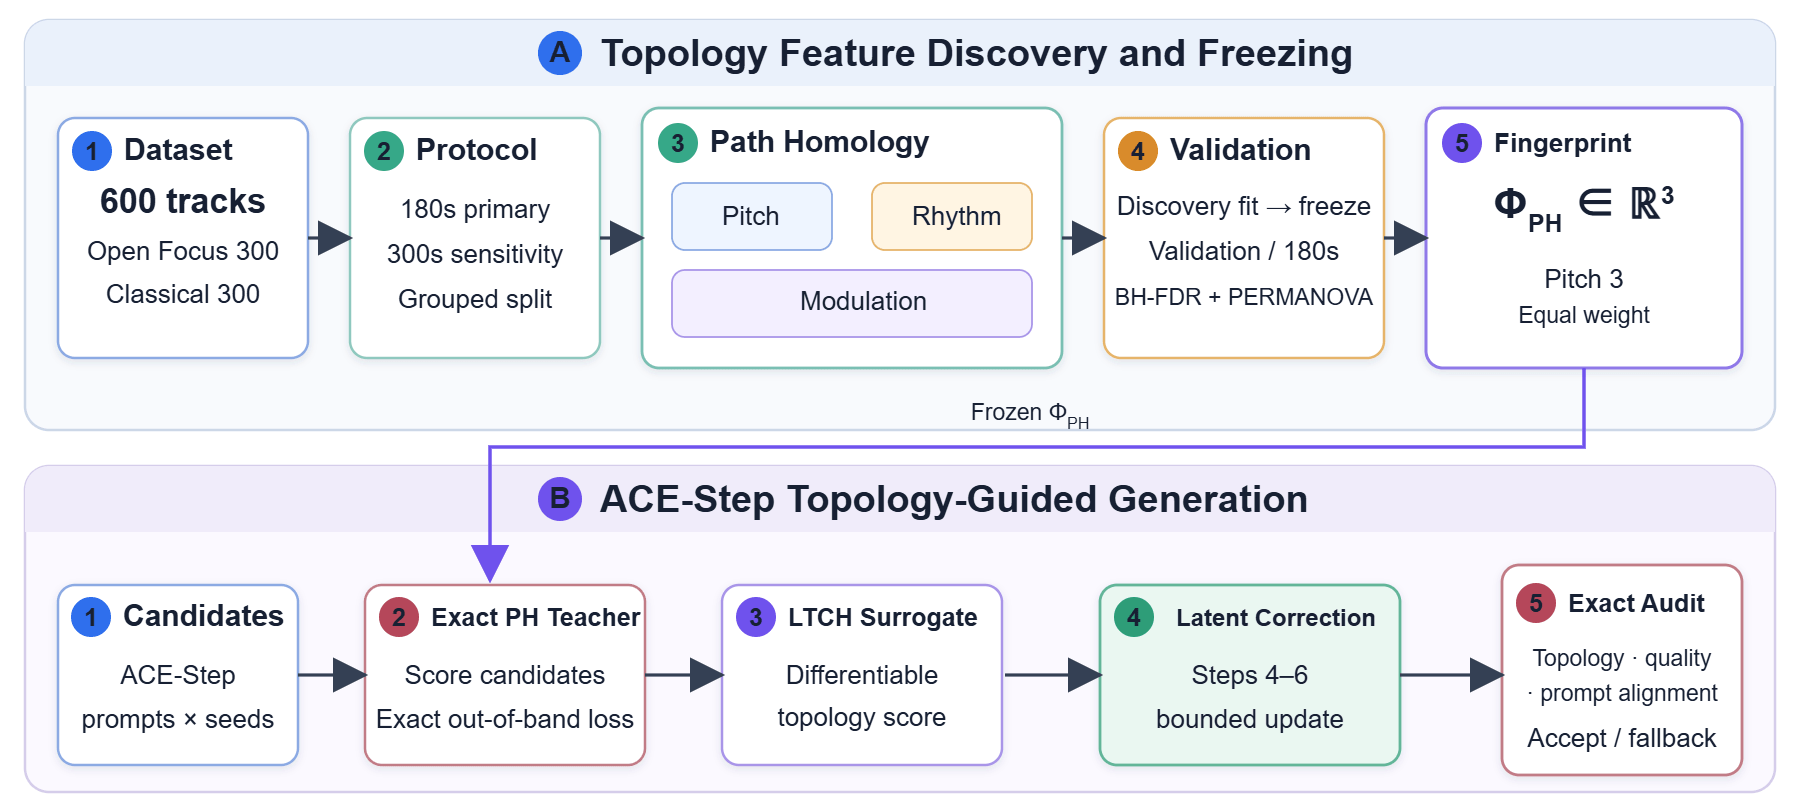
\includegraphics[width=\textwidth]{fig/p1.png}
    \caption{整体分析和应用框架。}
    \label{fig:p1}
\end{figure}

% Key Contributions

本研究的主要贡献总结如下：

\begin{itemize}
  \item 构建了保留转移方向的多尺度分析框架，通过将音乐状态转换表示为有向图，利用 GLMY 路径同调与持续路径同调分析音乐拓扑特征，并对 Open Focus--Classical 的观察性差异进行评估。
  \item 提出了相位提升环表示（phase-lifted recurrence graph representation），用跨周期同相位复现定义六相位有向环的边权，并以最弱边的持续阈值刻画闭环强度。
  \item 按``discovery 拟合与冻结---validation/180s 主要评估---validation/300s 同曲目敏感性检验''组织证据，并冻结由 Pitch、Acoustic phase 与 Chroma phase 构成的 $18$ 维拓扑指纹。
  \item 提出并训练了潜空间拓扑代理网络（LTSN），学习从 ACE-Step 潜变量到冻结拓扑指纹的可微近似，为采样期潜变量校正提供梯度。
  \item 构建了一个来源与逐曲许可可审计的双尺度语料库，包含 300 首 Open Focus 与 300 首 Classical 音乐，每首提供 180s 和 300s 两种分析片段。获取地址 \url{https://huggingface.co/datasets/fisheryv/open-focus-classical-600}
  \item 将拓扑特征发现过程中使用的代码封装成了一个 Python 库，名为 \texttt{pyglmy}，可在 \url{https://github.com/fisheryv/pyglmy} 上获取。
\end{itemize}

% 本研究完整的可复现代码已上传至 \url{https://github.com/fisheryv/glmy_focus_music}。

\section{Related Work}

\subsection{音乐拓扑分析}

Tonnetz 是音乐几何表示的重要历史来源之一，其后续推广可用于表达音级、音程与时间关系 \cite{Yust2020}。Mazzola 的 \emph{The Topos of Music} 则从范畴、模和拓扑等角度建立了更广泛的数学音乐理论框架 \cite{Guerino2017}。这些工作说明，音乐关系可以被组织为空间或代数结构，但它们并不直接给出本文所需的有向时序统计。

拓扑数据分析（Topological Data Analysis, TDA）中的持续同调通过一族过滤复形追踪拓扑特征随尺度的出现与消失 \cite{Edelsbrunner2002}。其中，$H_0$ 描述连通分支，$H_1$ 描述环，$H_2$ 描述二维空腔；持续图 \cite{David2007} 和 barcode \cite{Carlsson2004} 是同一持续信息的常用摘要形式。在音乐研究中，Sethares 与 Budney 展示了音高、音程和节奏数据中可由拓扑方法揭示的循环结构 \cite{Sethares_2014}；Alcalá-Alvarez 与 Padilla-Longoria 提出了从乐谱点集到单纯复形的系统分析框架 \cite{Alberto2024}；Heo 等人进一步比较了不同网络距离对音乐持续同调结果的影响 \cite{Heo_2025}。这些研究共同表明，结果依赖于表示与距离的选择，不能把某一种拓扑摘要视为与表示无关的音乐本质。

然而，标准 Vietoris--Rips 复形具有`无向性''和``对称性''，这种局限使得它无法有效应用于有向图。为了解决有向图的同调计算问题，Alexander Grigor'yan、Yong Lin、Yuri Muranov 和 Shing-Tung Yau 提出路径复形（Path Complex）与路径同调（Path Homology） \cite{glmy2013, glmy2020}。Mijangos 等人曾将音程转移表示为图并用持续同调探索音乐风格差异 \cite{Martin2022}，Wei 也从拓扑与谱方法研究了乐器声学形状 \cite{Wei2024}。相较于 TDA，GLMY 路径同调在功能性音乐中的应用仍较少；本文将工作定位为这一方向的具体实证应用。

\subsection{扩散模型生成控制与拓扑约束}

目前，潜空间生成控制与拓扑约束还是一个非常前沿的课题。Hu 等人在 3D 形状潜扩散中加入拓扑感知约束 \cite{hu2024topologyawarelatentdiffusion3d}；TopoDDPM 使用持续同调表征辅助点云生成 \cite{DU2026109240}；TopoLiDM 则通过图神经网络(GNN) 提取拓扑保持的潜图表示来建模 LiDAR 点云 \cite{liu2025topolidmtopologyawarelidardiffusion}。这些方法说明拓扑摘要可以参与生成条件或损失设计，但研究对象、拓扑构造与评价终点均不同于本文的有向音乐路径同调。

在音乐生成控制方面，Zachary Novack 等人提出了 LatCHs 与 Selective TFG 纯潜空间引导方案 \cite{novack2026}。LatCHs 直接构建在潜扩散模型的中间层扩散特征之上，可以直接在潜空间内预测音乐的动态强度、音高曲线与节拍位置。Selective TFG 技术通过仅在特定选择的少数关键时间步施加 LatCHs 梯度引导，大幅缩短计算耗时。本文与这些工作的联系在于使用可微代理读取潜变量；区别在于代理目标来自冻结的 Path Homology 指纹，并且只有在独立资格检验通过后才允许进入采样器。

\section{数据集}

\subsection{数据来源}

本研究使用两组共 600 首独立音乐，源文件总时长为 $57.81$ 小时。所有纳入曲目均记录来源页面、逐曲许可、内容哈希与切分归属。

\textbf{Open Focus 组}：该组由 300 首音乐构成。候选主要来自当前 Jamendo API，标签体系与数据背景参考 MTG-Jamendo \cite{bogdanov2019mtg}；纳入条件包括可核验的 \verb|instrumental| 证据、\verb|focus,meditation| 相关标签、允许下载以及逐曲 Creative Commons 许可。最终清单覆盖 154 位艺术家和 263 张专辑，总时长 $29.50$ 小时。

\textbf{Classical 组}：该组用于提供来源明确的古典器乐比较基线，共计 300 首音乐，来自公共领域标记与学术共享记录：
\begin{itemize}
  \item 基础池的 95 首音乐来自 \href{https://archive.org/details/musopen-lossless-dvd}{Musopen Lossless DVD} 项目，来源条目标注为 Public Domain Mark 1.0。涵盖多位大师的钢琴奏鸣曲和弦乐四重奏。
  \item 扩展池来自 \href{https://doi.org/10.5281/zenodo.5120004}{MusicNet Zenodo} 记录 \cite{john_thickstun_2016_5120004}，该记录标注为 CC BY 4.0。排除 \verb|source=Musopen| 以及与基础池重复的作品后，按作曲家平衡选取 205 条。
\end{itemize}
最终 Classical 清单涵盖了从钢琴独奏到室内弦乐的多种编制，总时长为 $28.31$ 小时。

\subsection{数据切分与治理}

数据治理旨在降低来源、流派、艺人风格或混音技术等带来的混淆因素。每首曲目生成 180s 与 300s 两个尺度：180s 是主要分析尺度，300s 仅用于同曲目时长敏感性。切片优先取曲目中段；短于目标时长时保留整曲，不循环、不补零、不跨曲拼接。

切分在源曲目级完成一次，并应用于两个时长版本。每组均为 discovery 195 首、validation 60 首、holdout 45 首。Open Focus 按艺术家整组划分；Classical 按作曲家并结合重复作品检查进行划分，以避免同一创作者或同一作品跨集合。discovery 用于拟合变换与状态模型，validation/180s 用于主要评估，validation/300s 是同曲目敏感性；当前 holdout 只承担冻结流程与方向的操作性检查，不应视为独立外部验证。

\begin{table}[h]
\centering
\caption{数据集构成与分析角色}
\label{tab:dataset}
\begin{tabular}{lrrrrrll}
\toprule
组别 & 曲目数 & 总时长(h) & discovery & validation & holdout & 许可 & 角色 \\
\midrule
Open Focus & 300 & 29.50 & 195 & 60 & 45 & CC & 功能性参考 \\
Classical  & 300 & 28.31 & 195 & 60 & 45 & PDM/CC BY & 比较基线 \\
\midrule
合计       & 600 & 57.81 & 390 & 120 & 90 &  & 源曲目级分组切分 \\
\bottomrule
\end{tabular}
\end{table}

\subsection{数据预处理}

% 所有待分析音频在解析层首先被强制转码为单声道（Mono）与 22.05 kHz 的全局统一采样率，并以浮点 float32 精度载入系统。由于响度的波动极易被非线性的拓扑模型捕捉并误解为宏观状态的跃迁，我们强制引入了符合广播级标准的 EBU R128 双向 \verb|loudnorm| 规范算法，所有音频片段在此被强制削平至 $-15$ LUFS 的基准响度，并在最后级联了一道 $-1$ dBFS 的软限幅器（soft limiting），扫除瞬态音量毛刺带来的干扰。

在进入拓扑分析前，所有音乐片段经过固定的数字信号处理流程，以减小格式、声道和响度尺度差异。

音频统一解码为 22.05 kHz、单声道、float32 WAV。响度处理采用 Two-pass EBU R128 \verb|loudnorm|，目标为 $-15$ LUFS，并在最终采样率下施加 $-1$ dBFS 峰值上限。当前两组共 1,200 个片段（600 个 180s、600 个 300s）全部通过配置哈希、输出哈希、响度和峰值审计；最终响度范围为 $-15.1997$ 至 $-14.8035$ LUFS，最大样本峰值为 $0.888737$。

切片不按最大能量择优，以避免系统性偏向高能量内容。固定候选顺序为中心窗、左侧相邻窗、右侧相邻窗、起始窗和末端窗；只有当前候选触发静音条件时才依次回退，以保证每个切片均包含连续且有效的声学几何信息。

\section{拓扑特征发现与验证}

\subsection{理论基础}

本文将音乐视为一个随时间演化的动态系统。音乐的每一小段可以被表示为一个状态，整首音乐则可以表示为状态序列：
\[S=(s_1,s_2,\ldots,s_T),\quad s_t\in\mathbb R^d.\]

如果音乐状态从 $s_t$ 演化到 $s_{t+1}$，则可以构建一个有向转移关系。定义 $i \to j$ 的非自转移计数为：
\[N_{ij}=\sum_{t=1}^{T-1}
\mathbf 1(s_t=i,\ s_{t+1}=j,\ i\neq j),\]
状态 $i$ 的非自转移总数为：
\[N_i^{\text{out}}=\sum_{k\neq i}N_{ik}.\]
则 $i \to j$ 的边权重为非自转移条件概率，即离开状态 $i$ 的条件下，下一状态为 $j$ 的经验概率：
\[
w_{ij}
=
\frac{N_{ij}}{N_i^{\mathrm{out}}}
=
\frac{N_{ij}}{\sum_{k\neq i}N_{ik}},
\quad N_i^{\mathrm{out}}>0.\]
自转移仅用于描述统计，不进入 Path Homology 图；每个源状态只保留权重最高的 6 条出边。

经过状态离散化后，音乐片段可以表示为加权有向图：
\[G_X=(V,E,W).\]
其中 $V$ 是音乐状态集合，$E$ 是状态转移边，$W$ 是边权矩阵。

过滤图 $G_\tau$ 保留 $w_{ij}\ge\tau$ 的边；阈值从 $0.95$ 降至 $0.05$ 过程中边逐渐增加：
\[G_\tau=
\left(V,\{i\rightarrow j:w_{ij}\ge\tau\}\right), \qquad G_{0.95}\subseteq G_{0.90}\subseteq\cdots\subseteq G_{0.05}.\]

对允许的 $p$-路径 $e_{v_0\ldots v_p}$，GLMY 边界算子为：
\[
\partial e_{v_0\ldots v_p}=\sum_i(-1)^i e_{v_0\ldots\widehat{v_i}\ldots v_p},\]
令允许路径空间 $\Omega_p=\{a\in A_p:\partial a\in A_{p-1}\}$，%其中 $A_p$ 由允许的有向 $p$-路径张成%
则
\[H_p^{\mathrm{path}}(G)=
\frac{\ker(\partial_p|_{\Omega_p})}{\operatorname{im}(\partial_{p+1}|_{\Omega_{p+1}})},
\qquad \beta_p=\dim H_p^{\mathrm{path}}(G).
\]
持久图和 barcode 使用 $a=1-\tau$ 把降阈值过滤改写为递增参数。对 $a_i\le a_j$，持久秩不变量为
$$
\rho_p(a_i,a_j)=\operatorname{rank}\operatorname{im}
\left[H_p(G_{a_i})\longrightarrow H_p(G_{a_j})\right].
$$

\subsection{分析框架与方法}

本研究从音高、节奏和调制三个视角将音乐表示为有向图，然后采用 GLMY 路径同调分析，在固定阈值过滤下提取连通性、环结构、持续性、路径熵、复现性及图密度等描述子。三个视角的输入特征和时间分辨率不同，但共享同一分析算子：首先仅在 discovery/180s 上拟合预处理器与状态码本，将连续特征序列 $\mathbf{x}^{(v)}_t$ 量化为离散状态 $s^{(v)}_t$；随后由相邻有效状态的转移计数 $N^{(v)}_{ij}$ 构造条件转移概率
\[
P^{(v)}_{ij}=\frac{N^{(v)}_{ij}}{\sum_jN^{(v)}_{ij}}.
\]
对每个状态保留概率最高的前 $6$ 条非自环出边，并在冻结阈值 $\{0.50,0.60,0.70,0.80,0.90,0.95\}$ 上形成超水平过滤。GLMY 路径同调与图统计共同产生 20 个预设指标，覆盖状态占用、转移数量与熵、自转移、有向复现、密度、互惠性以及 $H_0/H_1$ 持续性。自转移比例由原始状态序列统计，不因路径同调图排除自环而丢失。

所有指标在 validation/180s 上进行主验证：每项指标先做两组 Kruskal--Wallis 检验并报告 $\epsilon^2=(H-k+1)/(N-k)$；预设的 Open Focus--Classical 对比使用双侧 Mann--Whitney $U$ 检验并报告 rank-biserial 效应量。两套结果分别在各视角预定义的 20 指标家族内作 BH-FDR 校正，确认性阈值统一为 $q\le0.05$。validation/300s 重复同一分析，用于同曲目时长敏感性分析。

\subsection{状态表征}

\paragraph{音高状态}
对每个节拍的 12 维 chroma 向量 $c_t$ 作 $L_1$ 归一化，
\[\widetilde c_t(k)=\frac{c_t(k)}{\sum_{r=0}^{11}c_t(r)+\varepsilon},\]
再映射到 Harte Tonnetz 的五度、小三度和大三度三个圆周：
\[
T(c)=\sum_{k=0}^{11}\widetilde c(k)
\begin{bmatrix}
\cos(7\pi k/6)\\ \sin(7\pi k/6)\\
\cos(3\pi k/2)\\ \sin(3\pi k/2)\\
\cos(2\pi k/3)\\ \sin(2\pi k/3)
\end{bmatrix}.
\]
在 discovery/180s 上按组等量抽取每组 $50,000$ 个有效节拍，拟合固定的 16 状态谐波码本\cite{10.1145/1178723.1178727}。
%低置信节拍按 $1.15$ 主峰比规则记为缺失，不另设缺失状态，也不跨缺失位置连接转移。

\paragraph{节奏状态}
固定使用 1s 窗和 0.5s 步长，对第 $n$ 个窗口构造
\[\mathbf r_n=[\mu_o,\sigma_o,\operatorname{max}_o,\rho_o,\mu_{IOI},\sigma_{IOI},BPM,\rho_b]^\mathsf T.\]
其中前四项描述起音包络及起音率，$\mu_{IOI}$ 与 $\sigma_{IOI}$ 描述起音间隔，$BPM$ 和 $\rho_b$ 分别表示局部速度与拍点率。事件不足时相应维度记为缺失，以 discovery 中位数 $m_j$ 填补后按 discovery 均值和标准差标准化：
\[
r'_{n,j}=\begin{cases}r_{n,j},&\text{有效},\\m_j,&\text{缺失},\end{cases}
\qquad
\widetilde r_{n,j}=\frac{r'_{n,j}-\mu_j}{\sigma_j}.
\]
每组等量抽取 $50,000$ 个 discovery 窗口，拟合并冻结 10 状态码本。

\paragraph{调制状态}
对 Mel 子带能量包络 $x_b[n]$ 使用 4s 窗和 2s 步长，计算并跨子带累加调制功率：
\[
P_t(f_m)=\sum_b\left|\sum_n w[n]x_b[n+tH]e^{-i2\pi f_mn/f_s}\right|^2,
\qquad
\widetilde P_t(f_m)=\frac{P_t(f_m)}{\sum_{0.5\le f\le45}P_t(f)}.
\]
在 0.5--45Hz 内得到 178 维相对 SMP 后，依次采用 Hellinger 映射、discovery 中位数/IQR 稳健标准化和共享 PCA-32：
\[
h_{tj}=\sqrt{\widetilde P_t(f_j)},\qquad
z_{tj}=\frac{h_{tj}-\operatorname{median}_D(h_{\cdot j})}
{Q_{0.75,D}(h_{\cdot j})-Q_{0.25,D}(h_{\cdot j})},
\qquad y_t=W_{32}(z_t-\mu_D).
\]
32 个主成分累计解释方差为 $0.821$。平衡抽样后拟合固定的 10 状态码本，并按原始 SMP 频谱质心由低到高排序。
%由于该 SMP-$K=10$ 表征是在既有 holdout 打开后提出，本视角定位为探索性 validation 分析，而非与音高、节奏等同的冻结确认性证据。


表~\ref{tab:local_view_representations} 概括了三个视角的差异。所有缺失值处理、标准化、降维和聚类参数均只由 discovery/180s 估计，随后冻结应用于 validation。

\begin{table}[htbp]
\centering
\setlength{\tabcolsep}{4pt}
\caption{局部拓扑三个视角的状态表征}
\label{tab:local_view_representations}
\begin{tabular}{llll}
\toprule
视角 & 时间单元 & 连续表征 & 冻结状态模型 \\
\midrule
音高 & 节拍同步 & 12 维 Chroma $\rightarrow$ 6 维 Tonnetz & MiniBatch K-means，$K=16$ \\
节奏 & 1s 窗、0.5s 步长 & 8 维起音、IOI、BPM与拍点特征 & MiniBatch K-means，$K=10$ \\
调制 & 4s 窗、2s 步长 & 178 维相对 SMP $\rightarrow$ Hellinger $\rightarrow$ PCA-32 & MiniBatch K-means，$K=10$ \\
\bottomrule
\end{tabular}
\end{table}

\subsection{验证结果}

表~\ref{tab:local_view_summary} 汇总主验证与跨时长结果；完整 20 指标统计见附表~\ref{tab:pitch_topology}--\ref{tab:modulation_rank_biserial}。效应量及 180s/300s 稳定性见图~\ref{fig:pitch_effect_size}--\ref{fig:modulation_duration_stability}。

\begin{table}[htbp]
\centering
\setlength{\tabcolsep}{3pt}
\caption{局部拓扑视角的主要验证结果}
\label{tab:local_view_summary}
\begin{tabular}{lccp{5.2cm}p{2cm}p{1.4cm}l}
\toprule
视角 & 180s FDR & 跨时长稳定 & 主要组间方向 & $H_0$ & $H_1$ & 证据等级 \\
\midrule
音高 & 13/20 & 13 & Classical 覆盖与转移更多；Open Focus 状态保持、复现和音高互惠性更高 & 稳定组间差异 & 不支持 & 确认性 \\
节奏 & 14/20 & 14 & Classical 覆盖、熵、密度和互惠性更高；Open Focus 自转移与复现更高 & 稳定组间差异 & 不支持 & 确认性 \\
调制 & 5/20 & 4 & Open Focus 状态和绝对边更多，但密度与互惠性更低 & 无跨时长稳定结论 & 不支持 & 探索性 \\
\bottomrule
\end{tabular}
\end{table}

\begin{figure}[htbp]
    \centering
    \begin{minipage}{0.5\textwidth}
        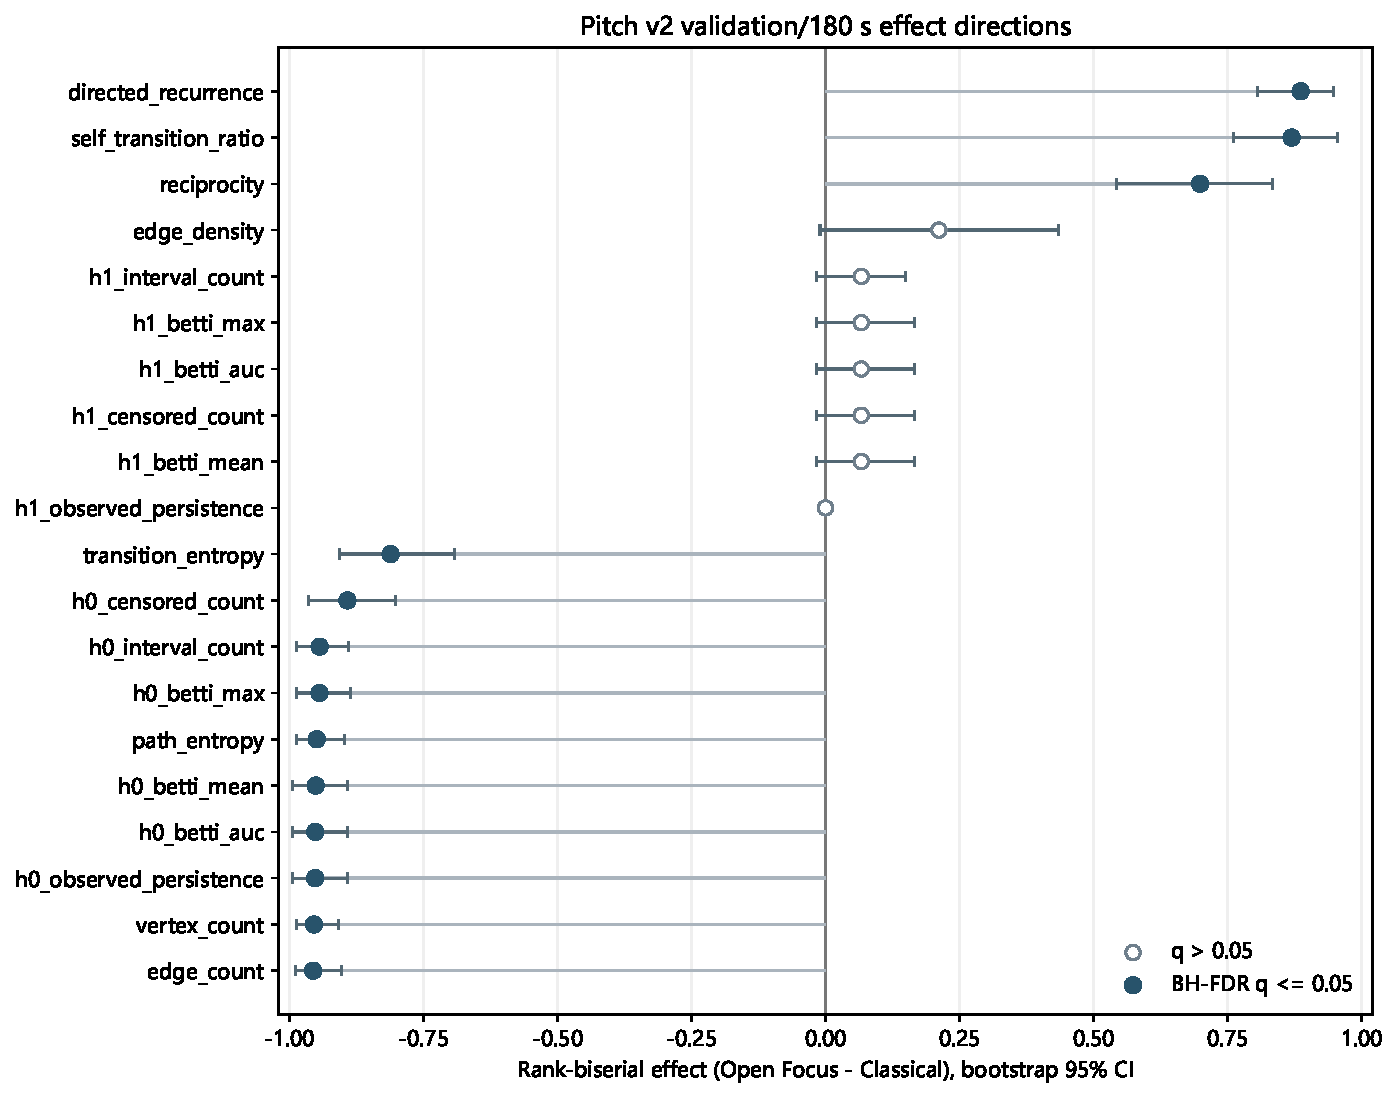
\includegraphics[width=\textwidth]{fig/pitch_v2_effect_sizes.pdf}
        \caption{音高 rank-biserial 效应量对比}
        \label{fig:pitch_effect_size}
    \end{minipage}
    \hfill
    \begin{minipage}{0.46\textwidth}
        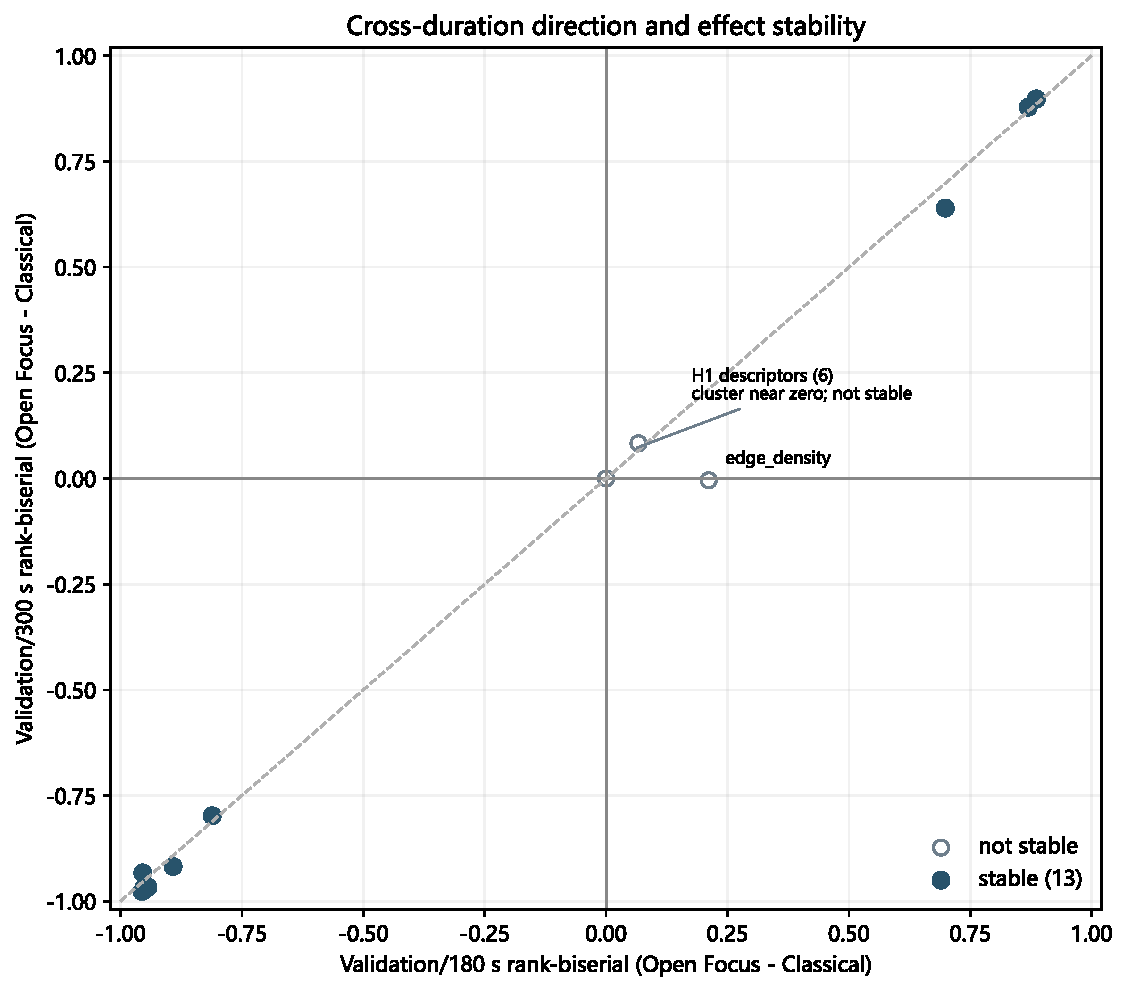
\includegraphics[width=\textwidth]{fig/pitch_v2_duration_stability.pdf}
        \caption{音高跨时长稳定性图}
        \label{fig:pitch_duration_stability}
    \end{minipage}
\end{figure}

\begin{figure}[htbp]
    \centering
    \begin{minipage}{0.5\textwidth}
        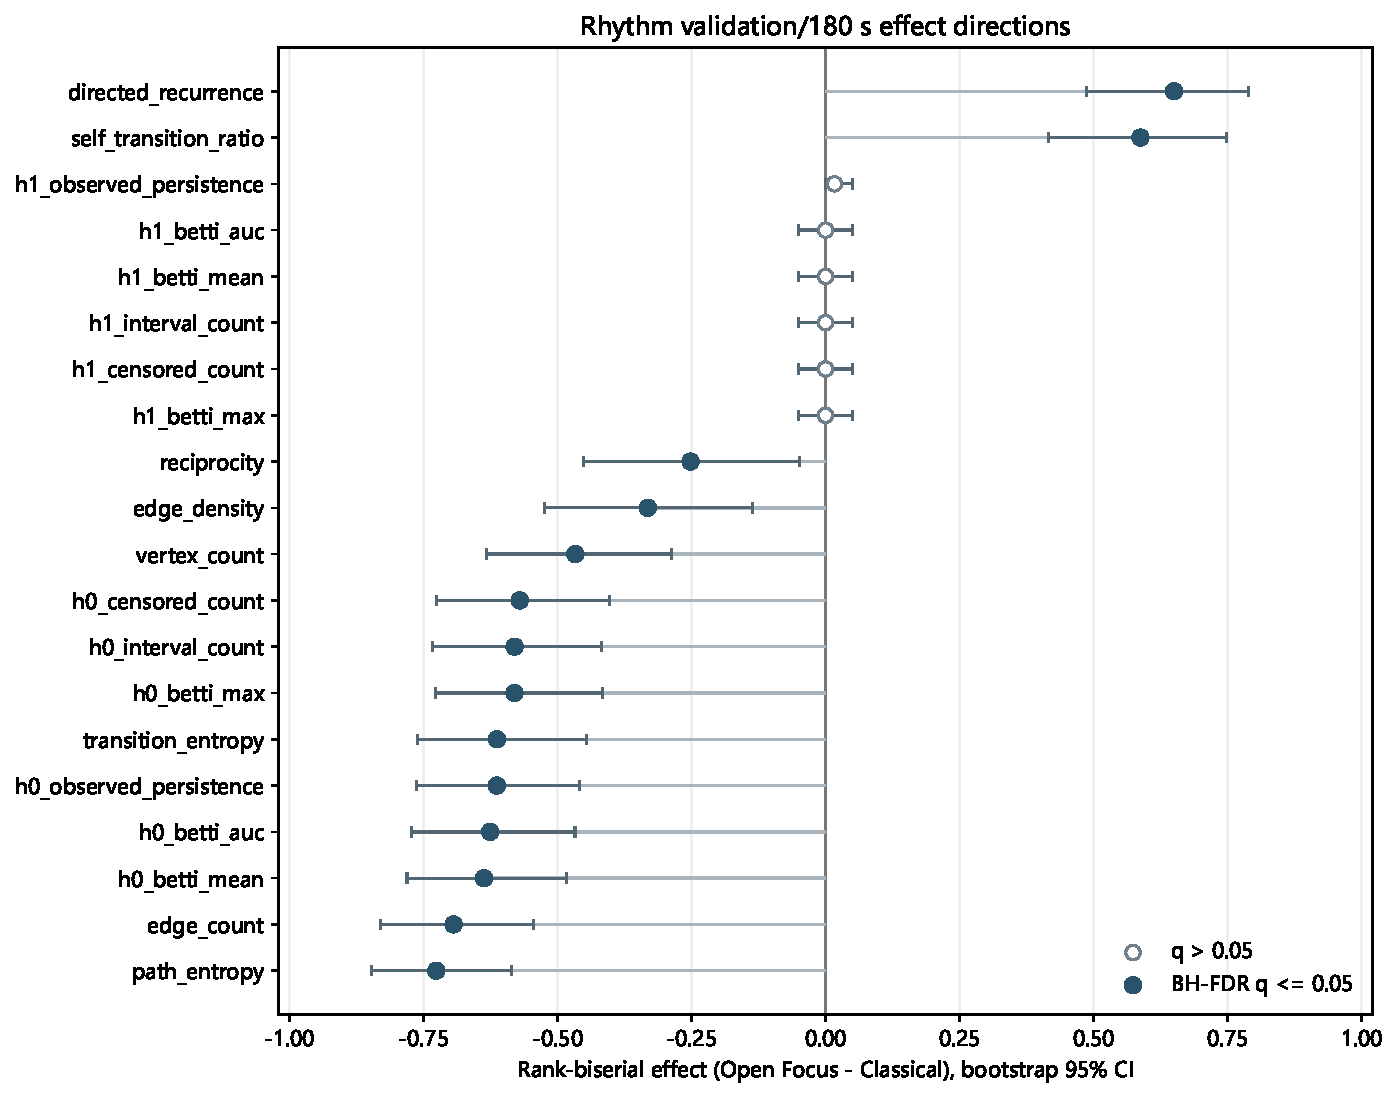
\includegraphics[width=\textwidth]{fig/rhythm_effect_sizes.pdf}
        \caption{节奏 rank-biserial 效应量对比}
        \label{fig:rhythm_effect_size}
    \end{minipage}
    \hfill
    \begin{minipage}{0.46\textwidth}
        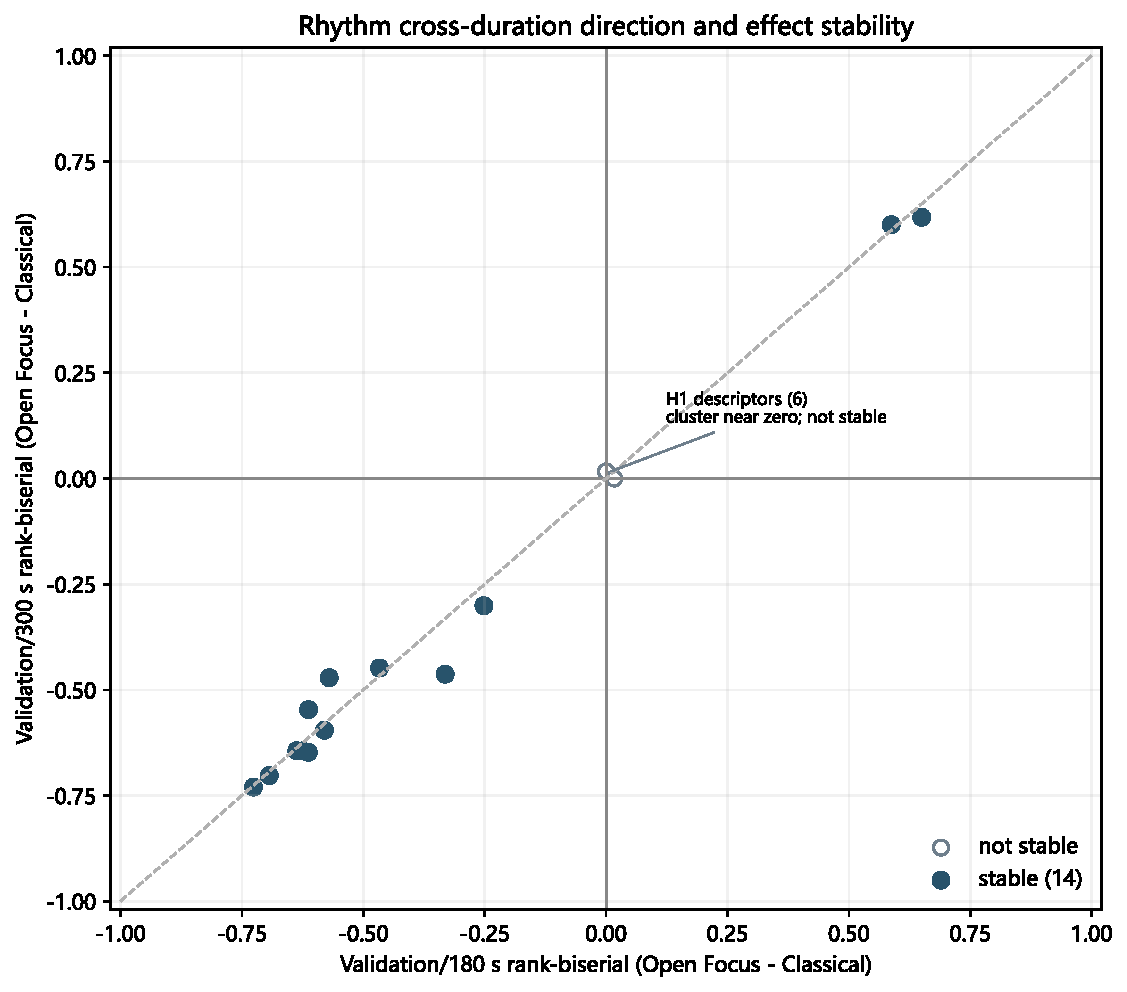
\includegraphics[width=\textwidth]{fig/rhythm_duration_stability.pdf}
        \caption{节奏跨时长稳定性图}
        \label{fig:rhythm_duration_stability}
    \end{minipage}
\end{figure}

\begin{figure}[htbp]
    \centering
    \begin{minipage}{0.5\textwidth}
        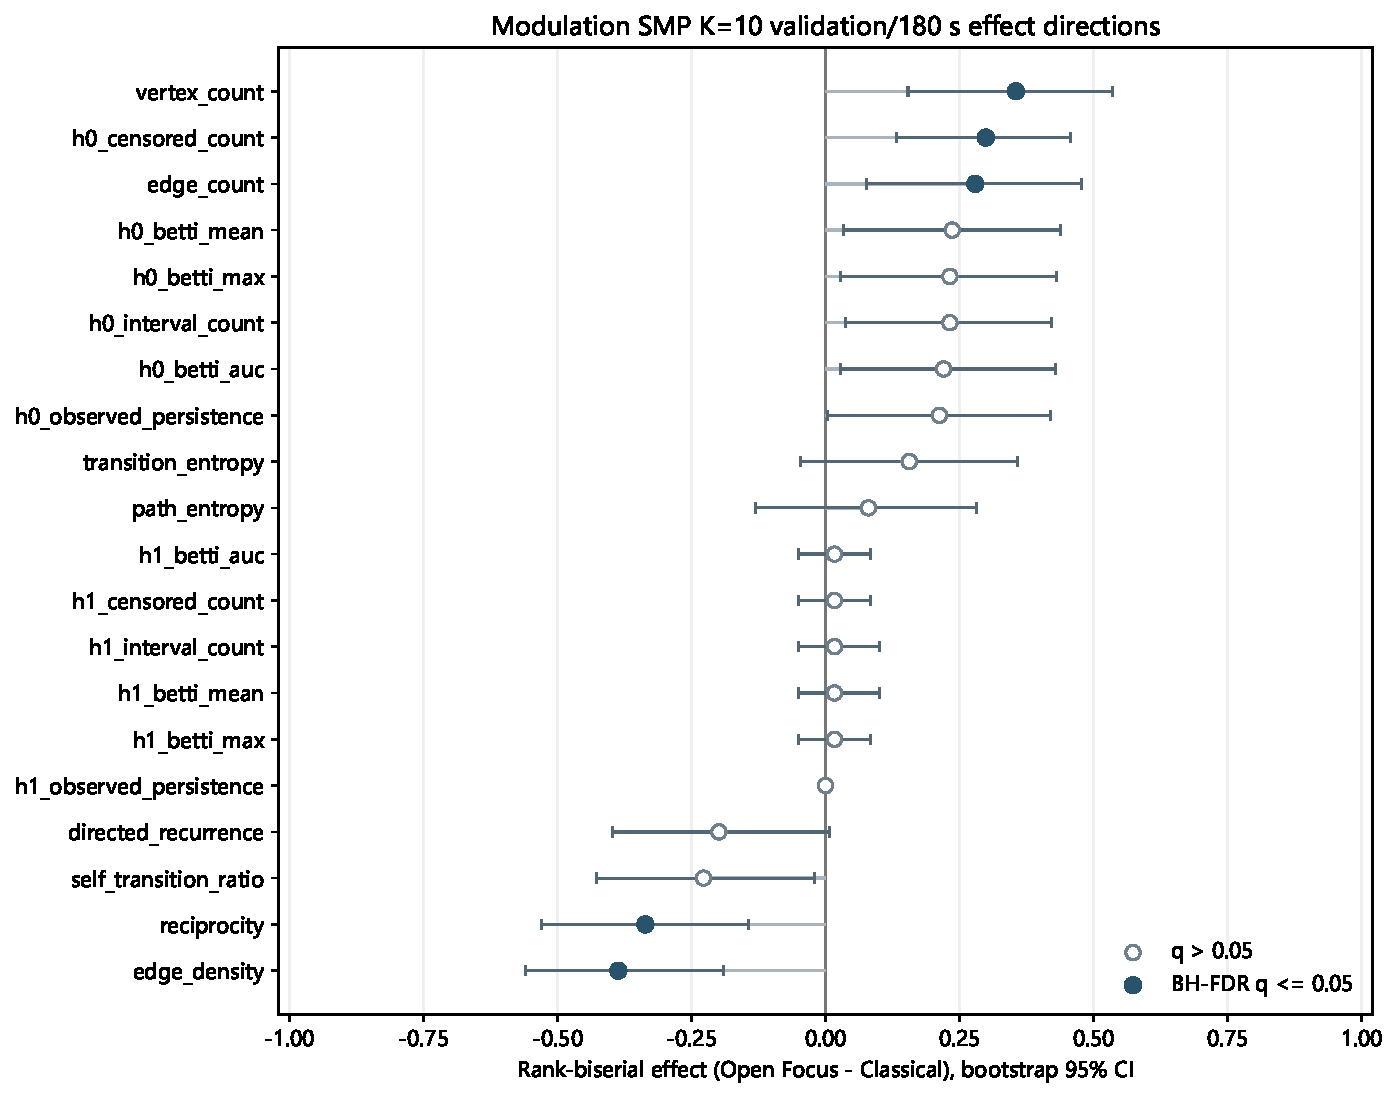
\includegraphics[width=\textwidth]{fig/modulation_smp_effect_sizes.pdf}
        \caption{调制 rank-biserial 效应量对比}
        \label{fig:modulation_effect_size}
    \end{minipage}
    \hfill
    \begin{minipage}{0.46\textwidth}
        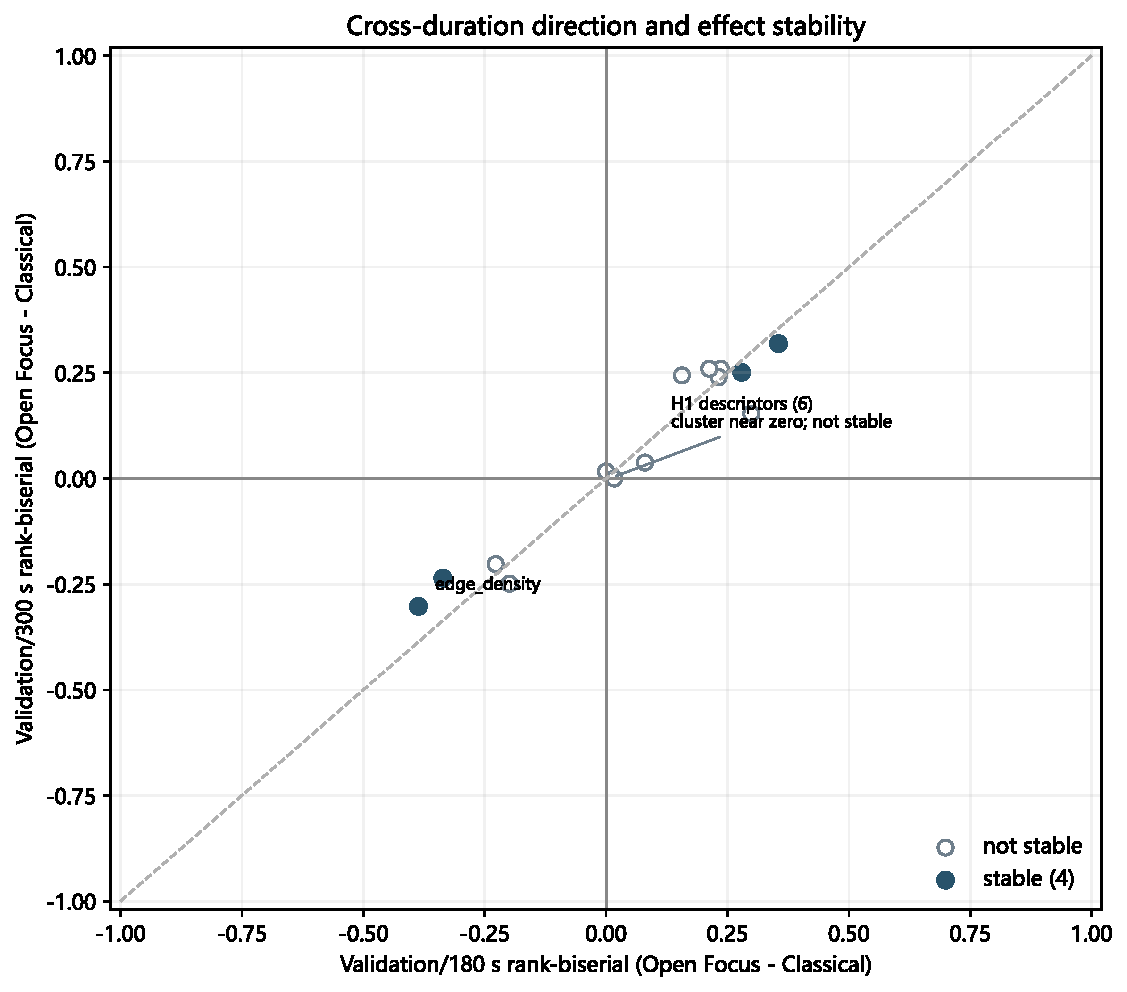
\includegraphics[width=\textwidth]{fig/modulation_smp_duration_stability.pdf}
        \caption{调制跨时长稳定性图}
        \label{fig:modulation_duration_stability}
    \end{minipage}
\end{figure}

音高和节奏视角呈现共同的组织模式：Classical 通常占用更多局部原型、形成更多有向边，并具有更高的路径熵与转移熵；Open Focus 则表现出更高的自转移比例和有向复现率。音高视角中，Classical 与 Open Focus 的状态数中位数分别为 $16$ 对 $10$、边数为 $70$ 对 $31$；节奏视角中相应数值分别为 $8$ 对 $7$、$36$ 对 $21$。与此同时，Open Focus 的音高自转移比例和有向复现率分别为 $0.631$ 和 $0.114$，高于 Classical 的 $0.322$ 和 $0.025$；节奏视角中的对应数值为 $0.662$、$0.265$ 与 $0.479$、$0.092$。因此，两类音乐的共同差异可概括为 Classical 的状态覆盖和转移多样性更广，而 Open Focus 的局部状态路径更集中、重复更强。

该共性不能外推到所有连接指标。音高互惠性在 Open Focus 中更高（$0.667$ 对 $0.522$），提示较强的相邻音高双向回返；节奏互惠性则在 Classical 中略高（$0.809$ 对 $0.769$），且其边密度也更高。因此，``Open Focus 局部复现更强''仅指自转移和既有有向路径的重复，不能改写为所有视角下的网络都更稠密或更双向。

\begin{figure}[htbp]
    \centering
    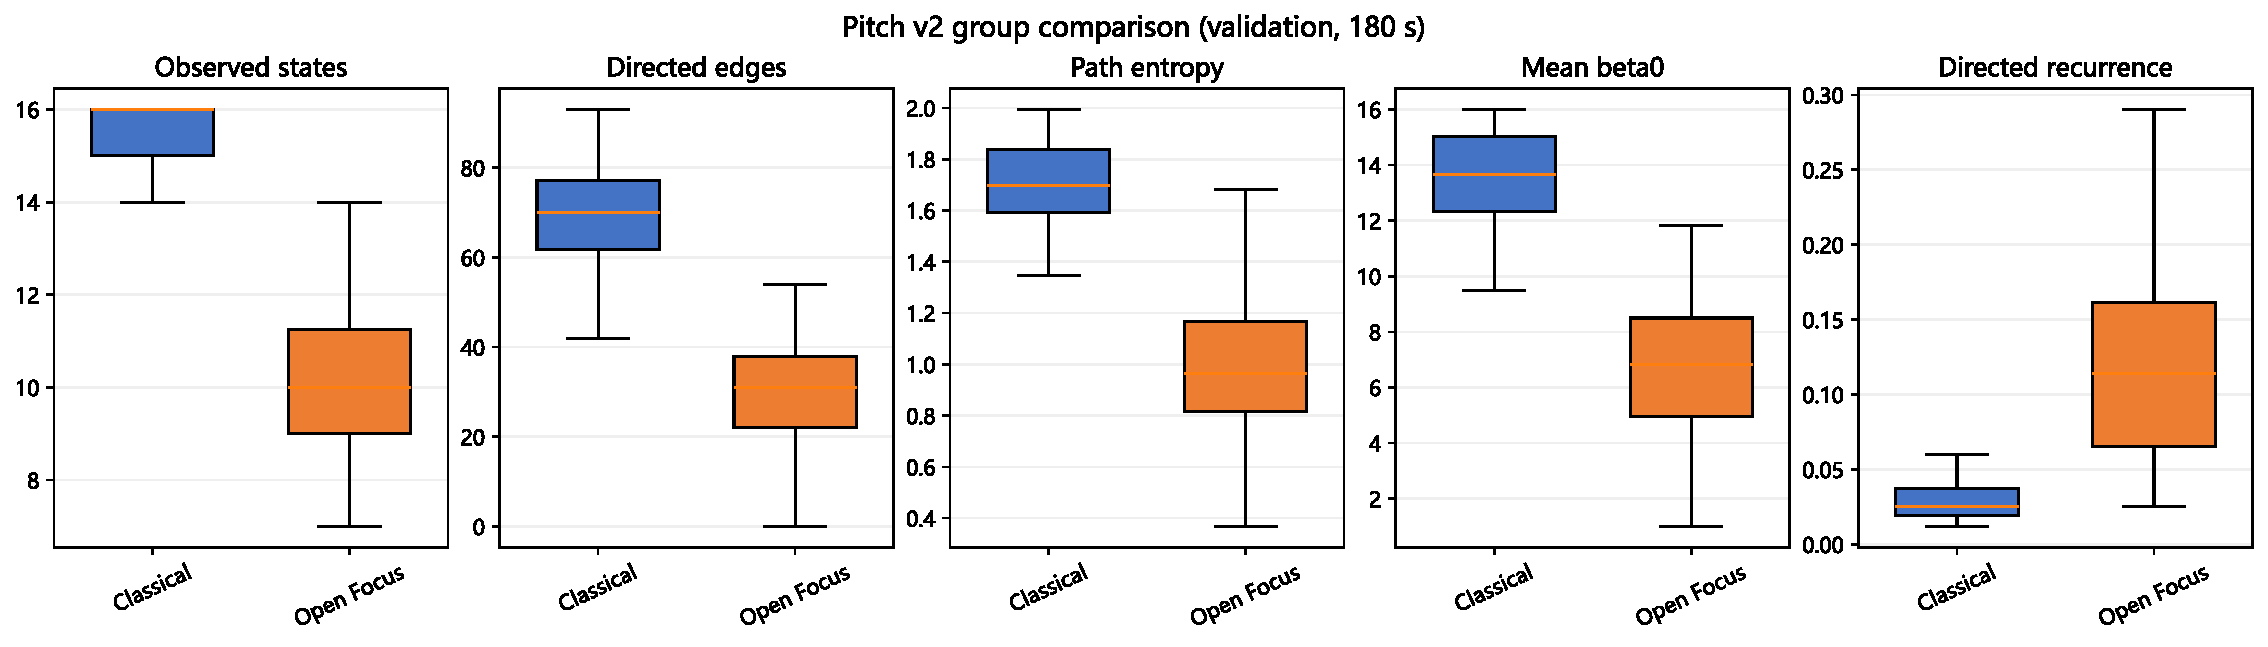
\includegraphics[width=\textwidth]{fig/pitch_v2_group_summary.pdf}
    \caption{音高视角下 Classical 与 Open Focus 的主要拓扑特征分布。}
    \label{fig:pitch_group_summary}
\end{figure}

\begin{figure}[htbp]
    \centering
    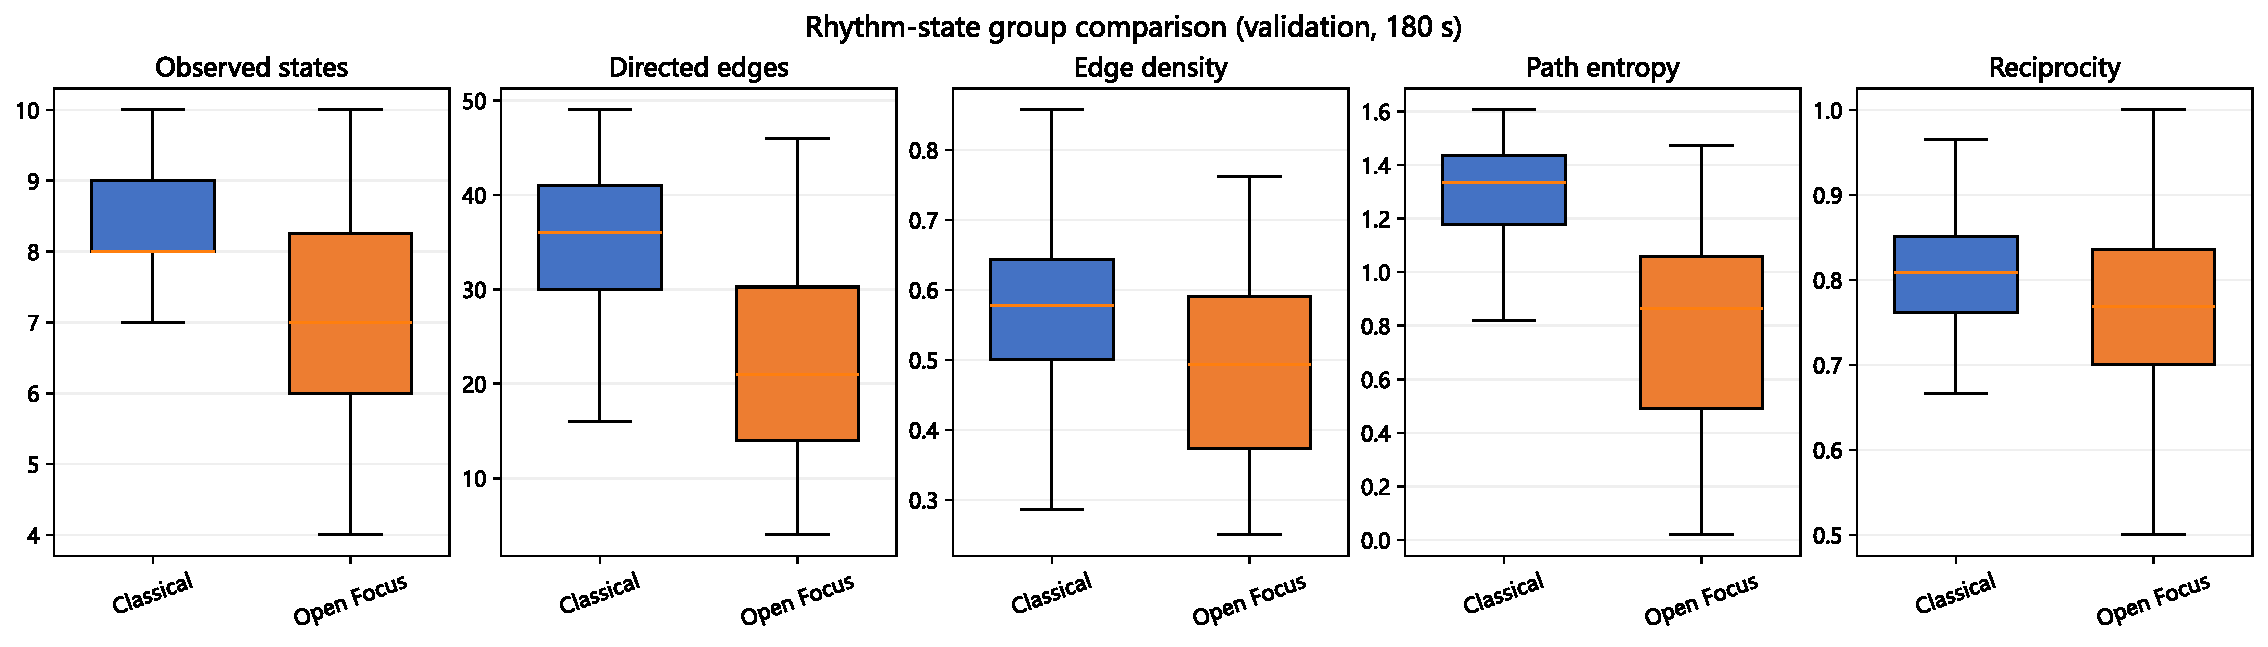
\includegraphics[width=\textwidth]{fig/rhythm_group_summary.pdf}
    \caption{节奏视角下 Classical 与 Open Focus 的主要拓扑特征分布。}
    \label{fig:rhythm_group_summary}
\end{figure}

\begin{figure}[htbp]
    \centering
    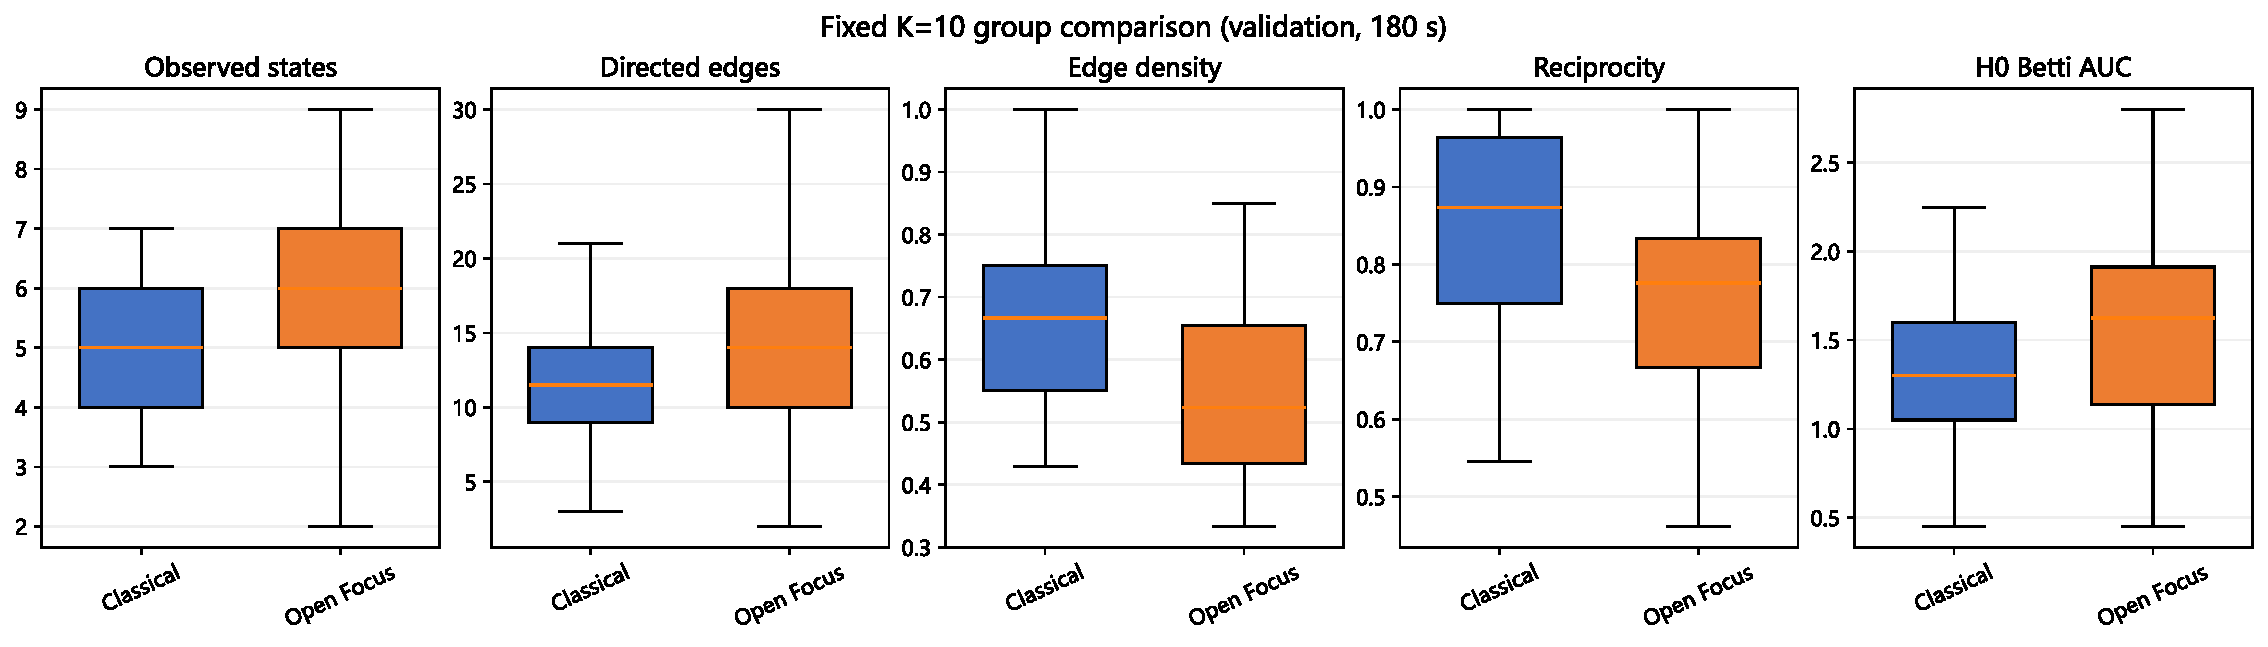
\includegraphics[width=\textwidth]{fig/modulation_smp_k10_group_summary.pdf}
    \caption{调制视角下 Classical 与 Open Focus 的主要拓扑特征分布。}
    \label{fig:modulation_group_summary}
\end{figure}

调制视角呈现不同于音高和节奏的模式。Open Focus 在共享 $10$ 状态 SMP 码本中访问更多原型并形成更多绝对边，状态数和边数中位数分别为 $6$ 和 $14$，高于 Classical 的 $5$ 和 $11.5$；但其边密度和互惠性分别为 $0.524$ 和 $0.776$，低于 Classical 的 $0.667$ 和 $0.873$。这表明 Open Focus 在当前 SMP 表征下覆盖更广，但连接相对于潜在边空间更稀疏、双向成对转移更少。四项跨时长稳定指标的 $\epsilon^2$ 为 $0.051$--$0.105$，rank-biserial 绝对值为 $0.279$--$0.386$，故该结果应作为效应有限的探索性解释层，而非已确认的核心指纹。

三个视角下的 betti 曲线见图~\ref{fig:pitch_betti_curves}--\ref{fig:modulation_betti_curves}。在同调层级上，音高和节奏的 $H_0$ 结果与状态覆盖差异一致：Classical 在冻结过滤过程中保留更多连通分量并经历更充分的分量合并。不过，$H_0$ 描述子同时受实际占用顶点数影响，应与状态数、边数和熵联合解释，不能单独表述为某一组具有更高或更优的拓扑复杂性。调制视角仅有 \verb|h0_censored_count| 在 180s 通过 FDR，且在 300s 不再显著（$q=0.159$），因而不形成稳定的 $H_0$ 结论。

三个视角均不支持稳定的组间 $H_1$ 差异。主阈值范围内，非零 $H_1$ 片段在音高视角为 Classical 2/60、Open Focus 6/60，在节奏视角均为 1/60，在调制视角为 2/60 和 3/60；六个预设 $H_1$ 指标的组中位数均为 0，且没有指标通过 180s 主分析 FDR。因此，局部视角的主要判别信息来自状态覆盖、转移集中性、局部复现和 $H_0$ 连通过程，而不是稳健的高阶环结构。

\begin{figure}[htbp]
    \centering
    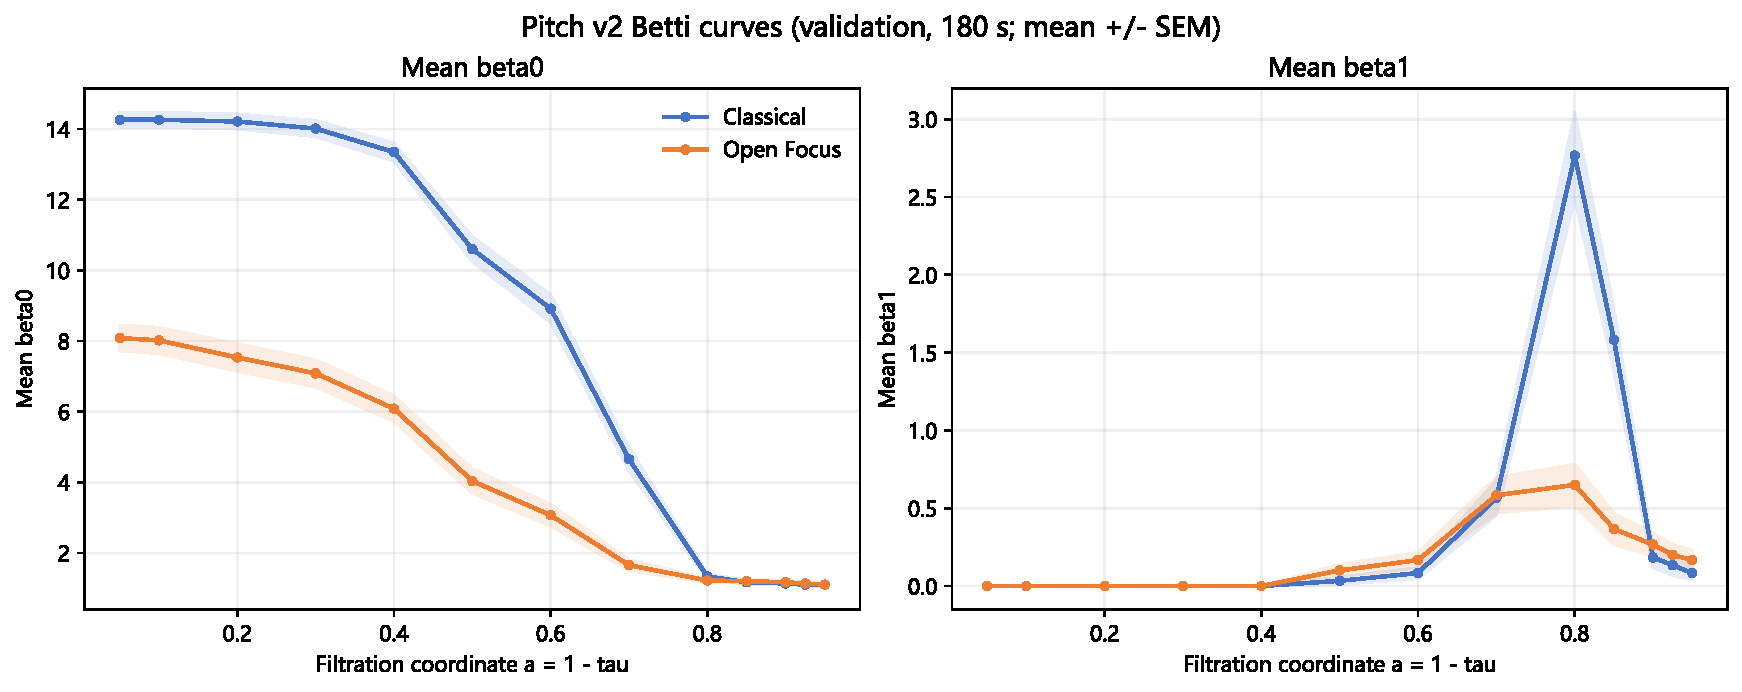
\includegraphics[width=\textwidth]{fig/pitch_v2_betti_curves.pdf}
    \caption{音高视角的 Betti 曲线。}
    \label{fig:pitch_betti_curves}
\end{figure}

\begin{figure}[htbp]
    \centering
    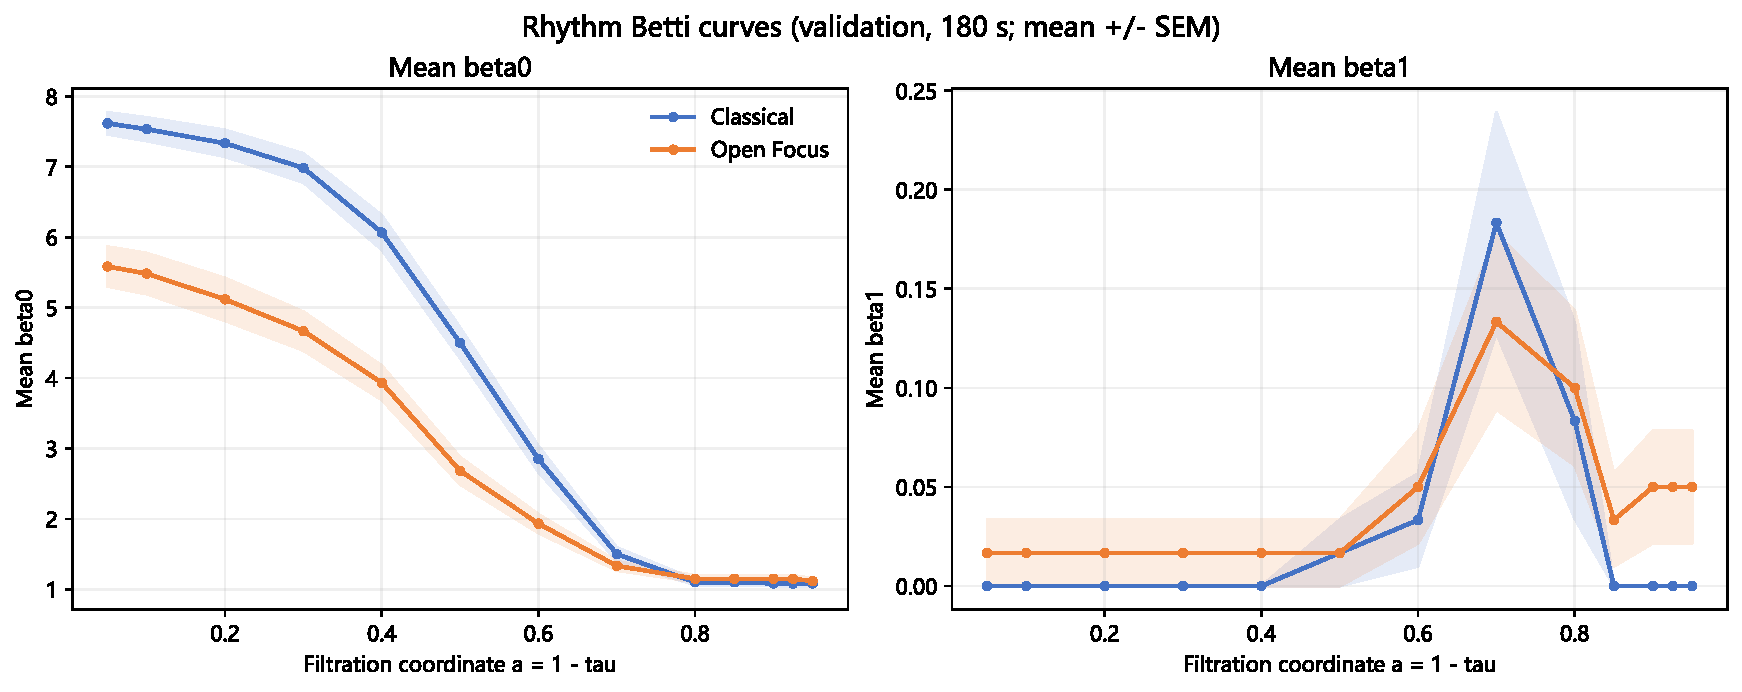
\includegraphics[width=\textwidth]{fig/rhythm_betti_curves.pdf}
    \caption{节奏视角的 Betti 曲线。}
    \label{fig:rhythm_betti_curves}
\end{figure}

\begin{figure}[htbp]
    \centering
    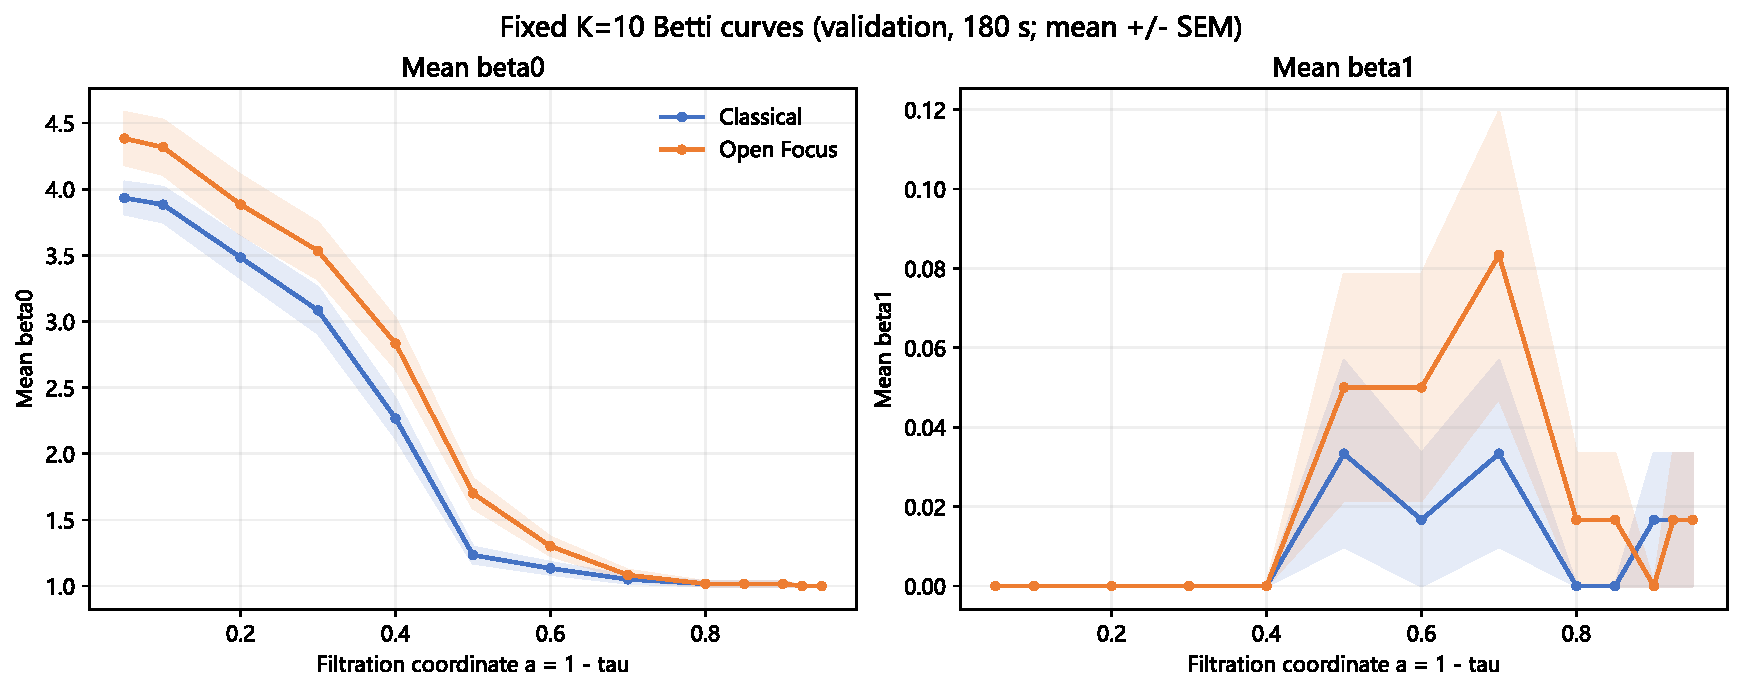
\includegraphics[width=\textwidth]{fig/modulation_smp_betti_curves.pdf}
    \caption{调制视角的 Betti 曲线。}
    \label{fig:modulation_betti_curves}
\end{figure}

\subsection{多视角融合与消融分析}
\label{sec:local_multiview_fusion}

音高、节奏和调制视角都以``局部状态---相邻转移---有向过滤''为共同接口，但分别描述和声位置、节奏组织与幅度调制轮廓。为检验这些信息能否在不构造高维笛卡尔积状态的前提下互补，本节将三组各 20 个预设拓扑描述子作为独立块进行后融合。整体流程如图~\ref{fig:local_multiview_fusion} 所示。

\begin{figure}[htbp]
  \centering
  \begin{tikzpicture}[
      node distance=1.5cm,
      block/.style={rectangle, draw, minimum width=3cm, minimum height=0.8cm, text centered},
      arrow/.style={->, >=stealth, thick}
  ]
      % Input nodes
      \node[block, text width=3.3cm] (P) {Pitch: 按拍 Tonnetz\\$K=16$};
      \node[block, text width=3.3cm, below of=P, yshift=-0.5cm] (R) {Rhythm: 1s / 0.5s\\$K=10$};
      \node[block, text width=3.3cm, below of=R, yshift=-0.5cm] (M) {Modulation: 4s / 2s\\PCA-32, $K=10$};
      
      % Mahalanobis blocks
      \node[block, text width=3cm, right of=P, xshift=2.5cm] (WP) {Discovery \\Mahalanobis block};
      \node[block, text width=3cm, right of=R, xshift=2.5cm] (WR) {Discovery \\Mahalanobis block};
      \node[block, text width=3cm, right of=M, xshift=2.5cm] (WM) {Discovery \\Mahalanobis block};
      
      % Fusion node
      \node[block, text width=2.5cm, right of=WR, xshift=2.5cm] (L) {Equal-block \\local fusion $L$};
      
      % Analysis node
      \node[block, text width=3.5cm, right of=L, xshift=2.5cm] (A) {PERMANOVA + leave-one-view-out + conditional residual};
      
      % Arrows
      \draw[arrow] (P) -- (WP);
      \draw[arrow] (R) -- (WR);
      \draw[arrow] (M) -- (WM);
      \draw[arrow] (WP) -- (L);
      \draw[arrow] (WR) -- (L);
      \draw[arrow] (WM) -- (L);
      \draw[arrow] (L) -- (A);
  \end{tikzpicture}
  \caption{多视角融合分析框架}
  \label{fig:local_multiview_fusion}
\end{figure}

\paragraph{冻结的块归一化与检验设计}
直接拼接会使有效维数或协方差尺度较大的视角主导距离。对视角 $v\in\{P,R,M\}$ 的 discovery/180s 描述子矩阵，先以 discovery 中位数填补缺失值并删除常量列，再估计均值 $\mu_v$ 与协方差 $\Sigma_v$。设其有效秩为 $r_v$，由 $\Sigma_v$ 的伪逆诱导白化矩阵 $W_v$，定义
\[
z_v(x)=\frac{(x-\mu_v)W_v}{\sqrt{r_v}},
\qquad W_vW_v^{\mathsf T}=\Sigma_v^{+}.
\]
音高、节奏和调制块的有效秩分别为 $13$、$13$ 和 $14$。除以 $\sqrt{r_v}$ 后，各块具有相近的期望平方距离尺度；三视角等权融合与任意两视角组合分别写为
\[
z_L(x)=\frac{1}{\sqrt{3}}[z_P(x)\Vert z_R(x)\Vert z_M(x)],
\qquad
z_{PR}(x)=\frac{1}{\sqrt{2}}[z_P(x)\Vert z_R(x)],
\]

主要检验为基于欧氏距离的 PERMANOVA，每个表示使用 $999$ 次标签置换。七个单视角或组合表示按时长分别作 BH-FDR 校正。为判断某一视角是否真正增加组间分离几何，在同一标签排列下计算
\[
\Delta F=F^{*}_{\mathrm{candidate}}-F^{*}_{\mathrm{baseline}},
\]
并对六个``完整融合相对单视角''及``加入一个视角''的比较按时长分别校正；只有 $\Delta F>0$ 且 $q\leq0.05$ 才判为正增量。另在 discovery/180s 上用其余两块拟合多输出岭回归 $\widehat f_v$，在 validation 中对残差
\[
R_v=Z_v-\widehat f_v(Z_{-v})
\]
再次进行 PERMANOVA，以诊断目标视角是否含有不能由其余两视角预测的组别信息。该条件残差检验不等价于因果分解，也不保证加入该视角后整体距离判别一定提高。

\paragraph{整体分离与组合消融}
表~\ref{tab:local_fusion_permanova} 显示，七种表示在两个时长下均能区分 Open Focus 与 Classical（原始置换 $p$ 均为 $0.001$，BH-FDR $q=0.001$）。完整融合在 180s 的 pseudo-$F$ 为 $6.27$，在 300s 为 $10.54$；但 180s 最强单视角是音高（$F^{*}=7.59$），300s 亦为音高（$F^{*}=18.19$）。因此，完整融合显著只能说明融合空间保留了组间差异，不能据此声称它优于最佳单视角。

\begin{table}[htbp]
\centering
\caption{局部三视角融合及组合消融的 PERMANOVA 结果}
\label{tab:local_fusion_permanova}
\setlength{\tabcolsep}{5pt}
\begin{tabular}{lrrrrr}
\toprule
表示 & 维数 & 180s $F^{*}$ & 180s $q$ & 300s $F^{*}$ & 300s $q$ \\
\midrule
音高（$P$） & 16 & 7.59 & 0.001 & 18.19 & 0.001 \\
节奏（$R$） & 16 & 6.47 & 0.001 & 10.24 & 0.001 \\
调制（$M$） & 17 & 4.13 & 0.001 & 4.24 & 0.001 \\
$P+R$ & 32 & 7.08 & 0.001 & 14.11 & 0.001 \\
$P+M$ & 33 & 6.17 & 0.001 & 10.69 & 0.001 \\
$R+M$ & 33 & 5.40 & 0.001 & 7.10 & 0.001 \\
$P+R+M$ & 49 & 6.27 & 0.001 & 10.54 & 0.001 \\
\bottomrule
\end{tabular}
\end{table}

\paragraph{融合空间的二维投影}
为直观展示完整融合表示中的样本关系，图~\ref{fig:local_fusion_pca} 使用仅在 discovery/180s 上拟合的 PCA，将 validation/180s 的 49 维融合坐标投影到前两个主成分。Classical 曲目主要分布在 PC1 正向且相对集中，Open Focus 整体偏向 PC1 负向并呈现更大的组内离散，但两组仍存在明显重叠。PC1 与 PC2 分别只解释 $4.8\%$ 和 $4.7\%$ 的方差，合计为 $9.5\%$；因此该图仅提供低维几何直觉，不参与 PERMANOVA 或配对增量检验。

\begin{figure}[htbp]
    \centering
    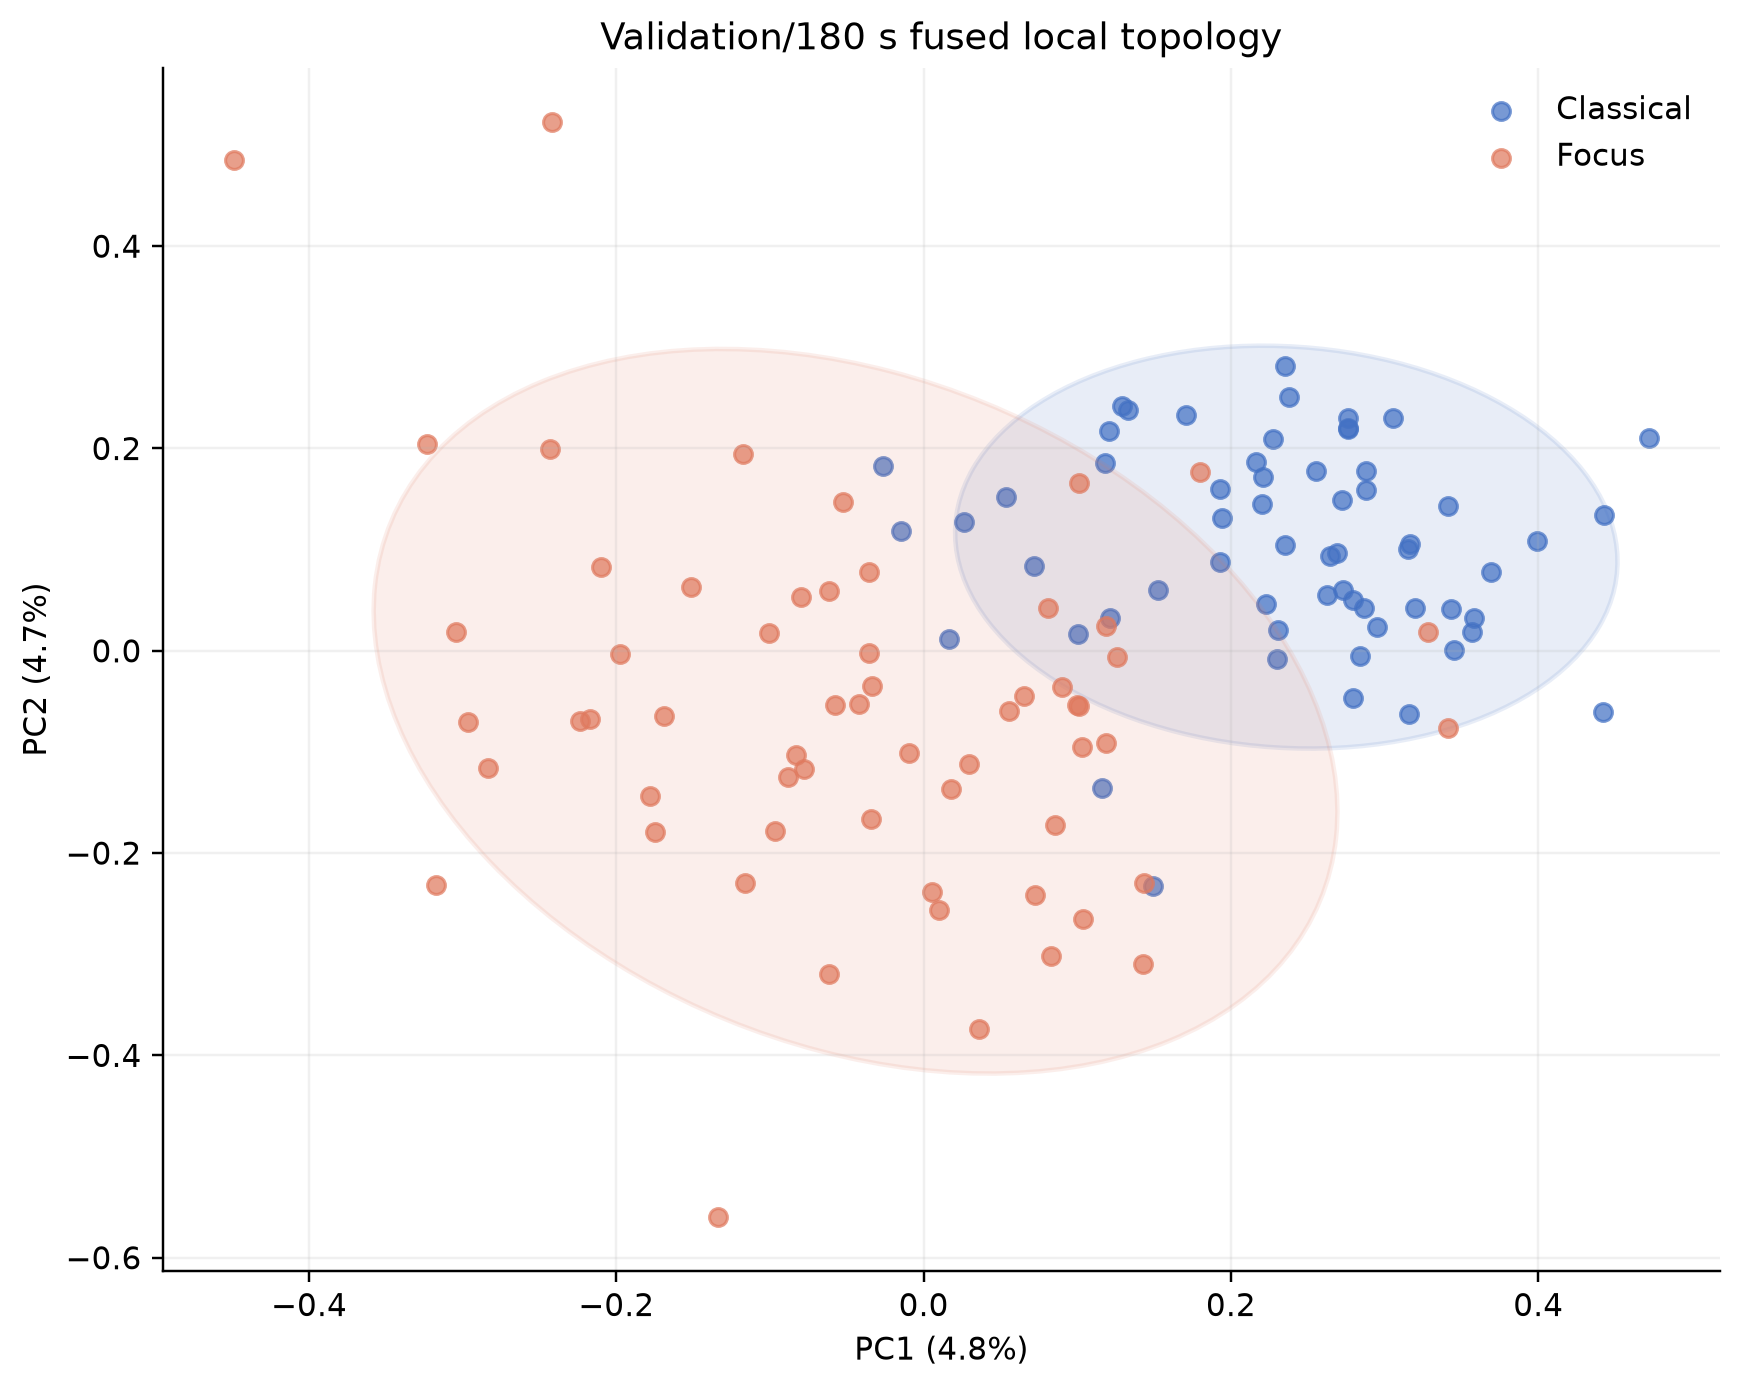
\includegraphics[width=0.78\textwidth]{fig/local_smp_k10_pca_validation_180.png}
    \caption{由 discovery/180s 拟合的 PCA 对 validation/180s 三视角融合表示的二维投影。每个点代表一首曲目；椭圆阴影表示以组内均值为中心、沿组内协方差主轴延伸 $1.96$ 个标准差的投影范围，并非 bootstrap 置信区间。}
    \label{fig:local_fusion_pca}
\end{figure}

\paragraph{增量与条件非冗余}
配对增量结果见图~\ref{fig:local_fusion_incremental}。在 180s 主分析中，完整融合相对音高的 $\Delta F=-1.32$（$q=1$），相对节奏为 $-0.205$（$q=1$）；相对调制虽为 $2.14$（$q=0.003$），但这仅说明融合优于较弱的调制单视角。留一视角消融中，向``节奏+调制''加入音高产生稳定正增量（180s：$\Delta F=0.864$，$q=0.003$；300s：$3.44$，$q=0.003$）。向``音高+调制''加入节奏在 180s 的增量仅为 $0.101$（$q=0.462$），而向``音高+节奏''加入调制反而为 $-0.814$（$q=1$）；二者均无正向增量证据。该结果将音高识别为当前等权距离中的主要分离块，而不支持``每增加一个视角都会增强组间几何''的假设。

\begin{table}[htbp]
\centering
\caption{局部三视角融合的配对 pseudo-$F$ 增量检验结果}
\label{tab:local_fusion_incremental}
\begin{tabular}{lrrrr}
\toprule
比较 & 180 s $\Delta F$ & 180s FDR & 300s $\Delta F$ & 300s FDR \\
\midrule
Full-Pitch & -1.32 & 1 & -7.65 & 1 \\
Full-Rhythm & -0.205 & 1 & 0.298 & 0.342 \\
Full-Modulation & 2.14 & 0.003 & 6.3 & 0.003 \\
Add Pitch to Rhythm+Modulation & 0.864 & 0.003 & 3.44 & 0.003 \\
Add Rhythm to Pitch+Modulation & 0.101 & 0.462 & -0.146 & 1 \\
Add Modulation to Pitch+Rhythm & -0.814 & 1 & -3.56 & 1 \\
\bottomrule
\end{tabular}
\end{table}

\begin{figure}[htbp]
    \centering
    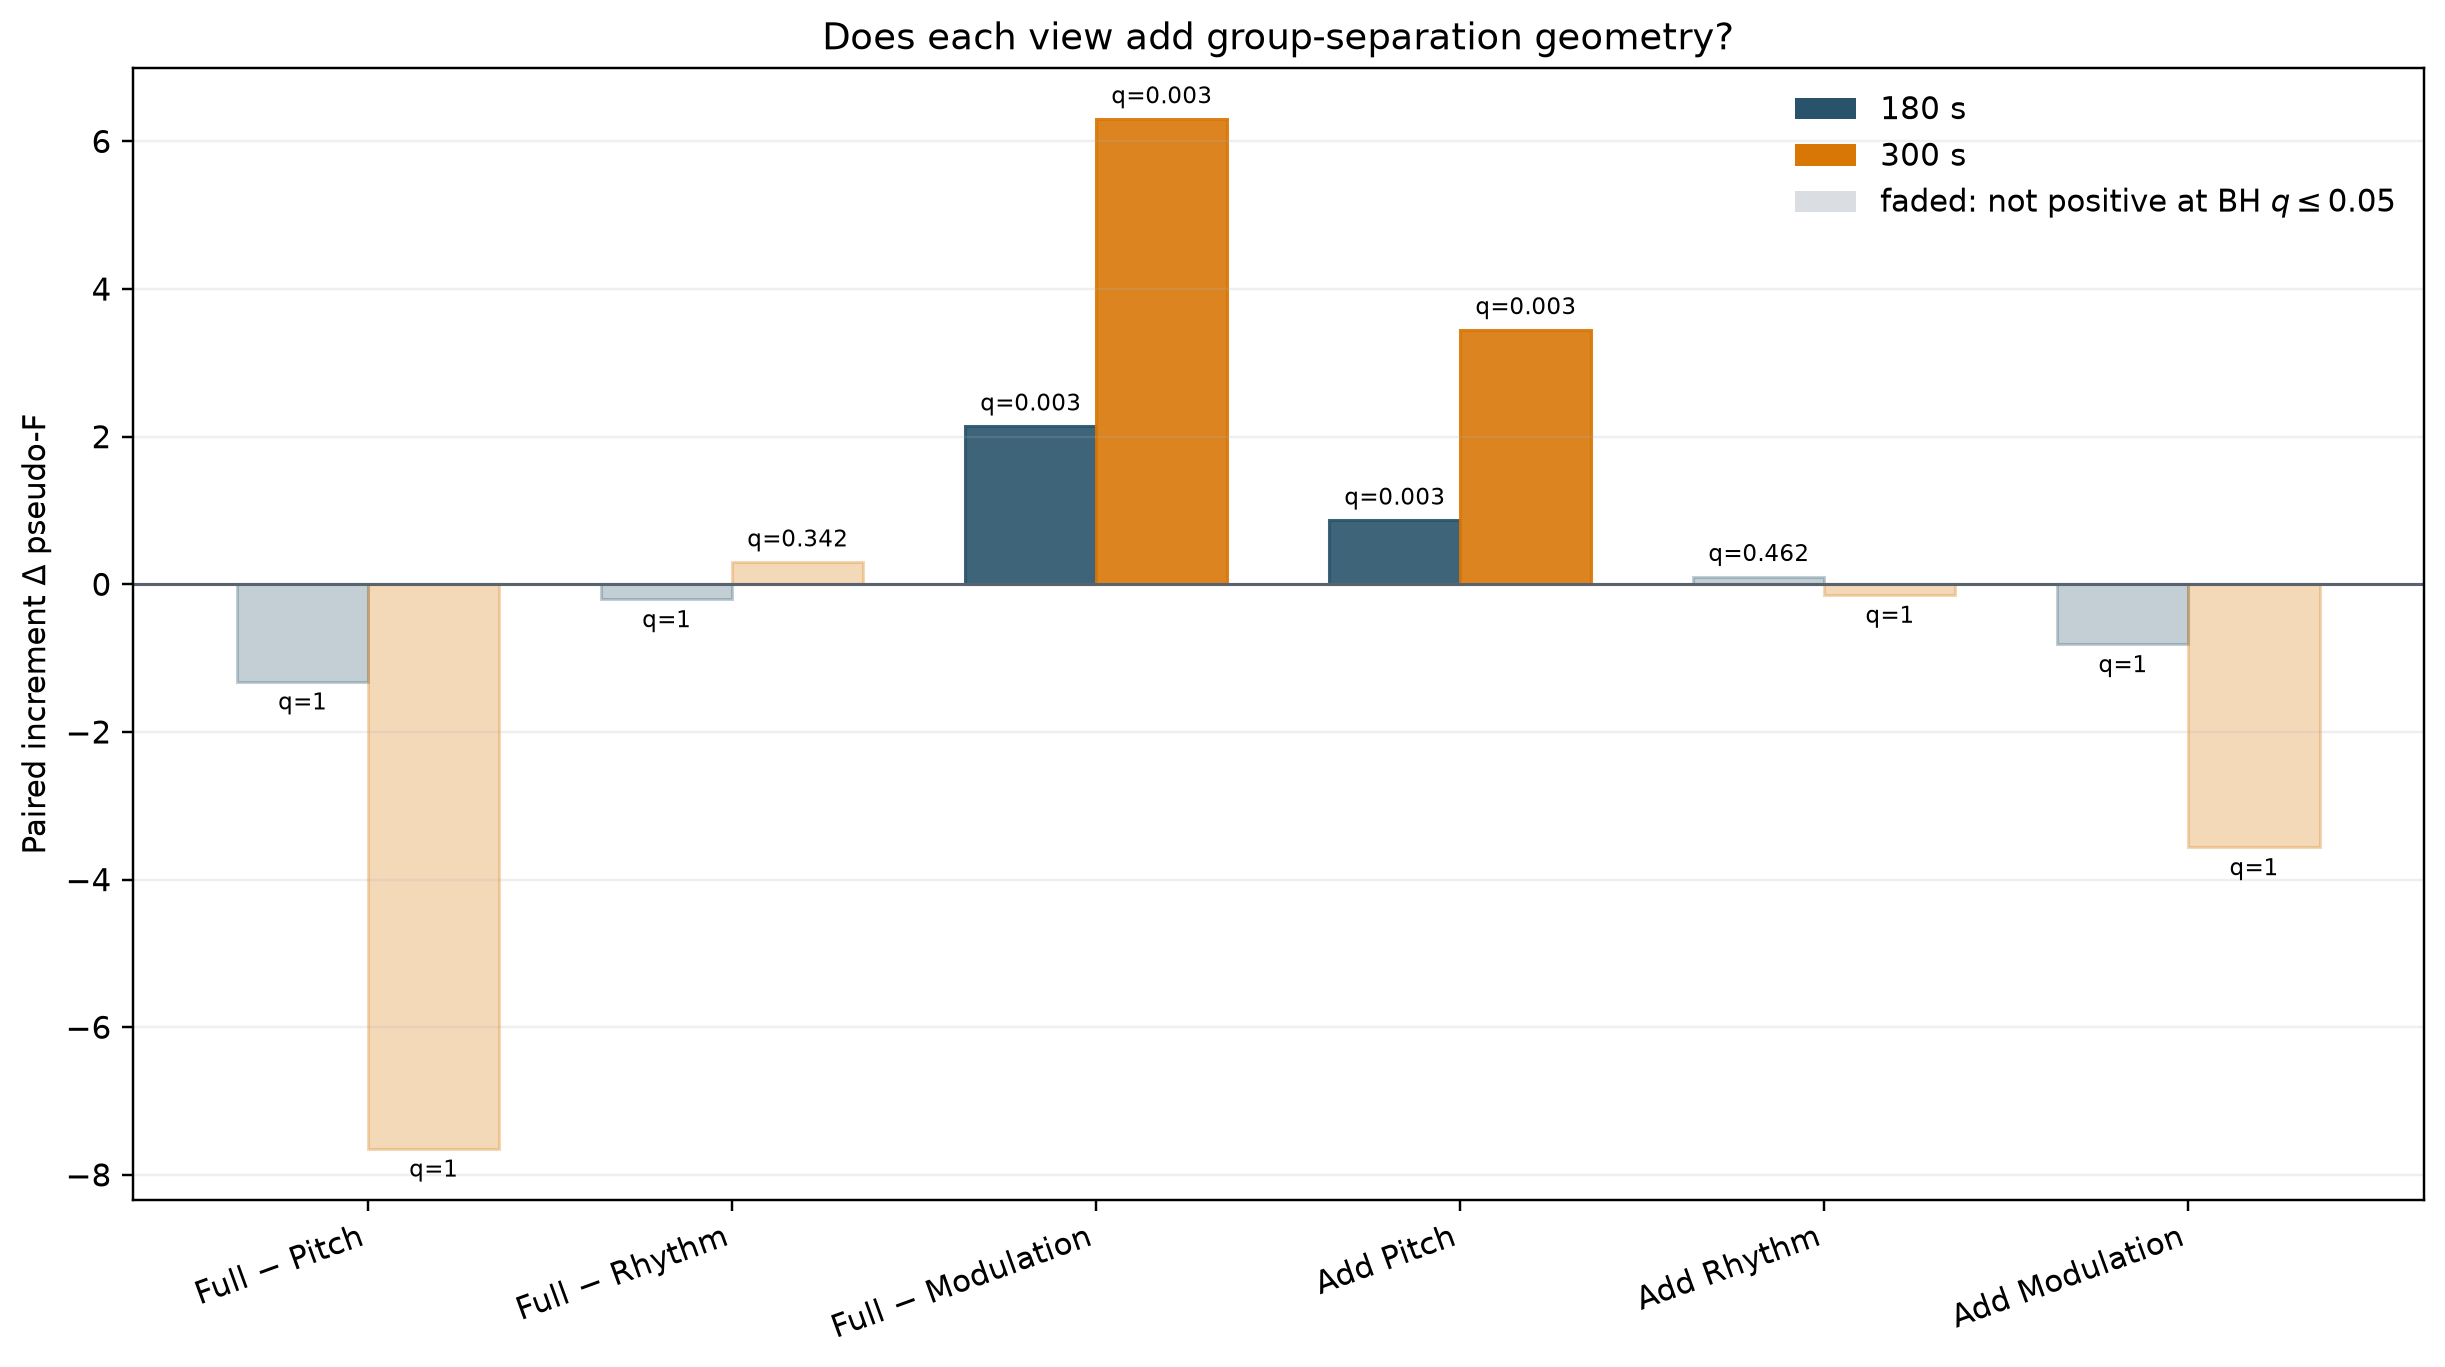
\includegraphics[width=\textwidth]{fig/local_smp_k10_incremental_tests.png}
    \caption{局部三视角融合的配对 pseudo-$F$ 增量检验。浅色柱表示未同时满足 $\Delta F>0$ 与 BH-FDR $q\leq0.05$；300s 仅作同曲目时长敏感性。}
    \label{fig:local_fusion_incremental}
\end{figure}

条件残差给出了不同但互补的问题答案。表~\ref{tab:local_fusion_residual} 中，三个视角的残差在 180s 均仍含显著组别结构；300s 方向也一致。然而，节奏和调制的 validation $R^2$ 接近零或为负，说明 discovery 上拟合的跨视角预测关系并未稳定推广。因而，这些结果支持三视角包含条件非冗余信息，但不能推导为每个视角都对等权融合产生可验证的正增量。

\begin{table}[htbp]
\centering
\caption{各局部视角在条件于其余两视角后的残差 PERMANOVA}
\label{tab:local_fusion_residual}
\setlength{\tabcolsep}{4pt}
\begin{tabular}{lrrrrr}
\toprule
目标视角 & 180s $F^{*}$ & 180s $q$ & validation $R^2$ & 300s $F^{*}$ & 300s $q$ \\
\midrule
音高 & 4.53 & 0.0015 & 0.0476 & 11.74 & 0.0015 \\
节奏 & 3.39 & 0.0015 & $-0.0089$ & 6.34 & 0.0015 \\
调制 & 2.22 & 0.0100 & 0.0034 & 1.88 & 0.0310 \\
\bottomrule
\end{tabular}
\end{table}

\paragraph{辅助分类及指标分歧}
作为辅助分析，在 discovery/180s 内部以五折交叉验证选择 $C$ 的 L2 logistic regression，冻结后应用于 validation；分类差异使用固定种子的 $1,000$ 次组内分层 bootstrap。完整融合在 180s 的 balanced accuracy、Macro-F1 和 AUROC 分别为 $0.967$、$0.967$ 和 $0.991$，音高单视角分别为 $0.925$、$0.925$ 和 $0.986$。完整融合相对音高的 balanced accuracy 增量为 $0.0417$，bootstrap 95\% CI 为 $[0.0165,0.0750]$。此外，在 $P+R$ 上加入调制后 balanced accuracy 增加 $0.0333$，95\% CI 为 $[0.0083,0.0667]$；但其距离增量为 $\Delta F=-0.814$、$q=1$。分类性能衡量逐曲判别，pseudo-$F$ 衡量组间距离相对组内离散的比例，两者可以不同方向变化，因此必须并列报告，不能只选择有利指标。

\begin{figure}[htbp]
    \centering
    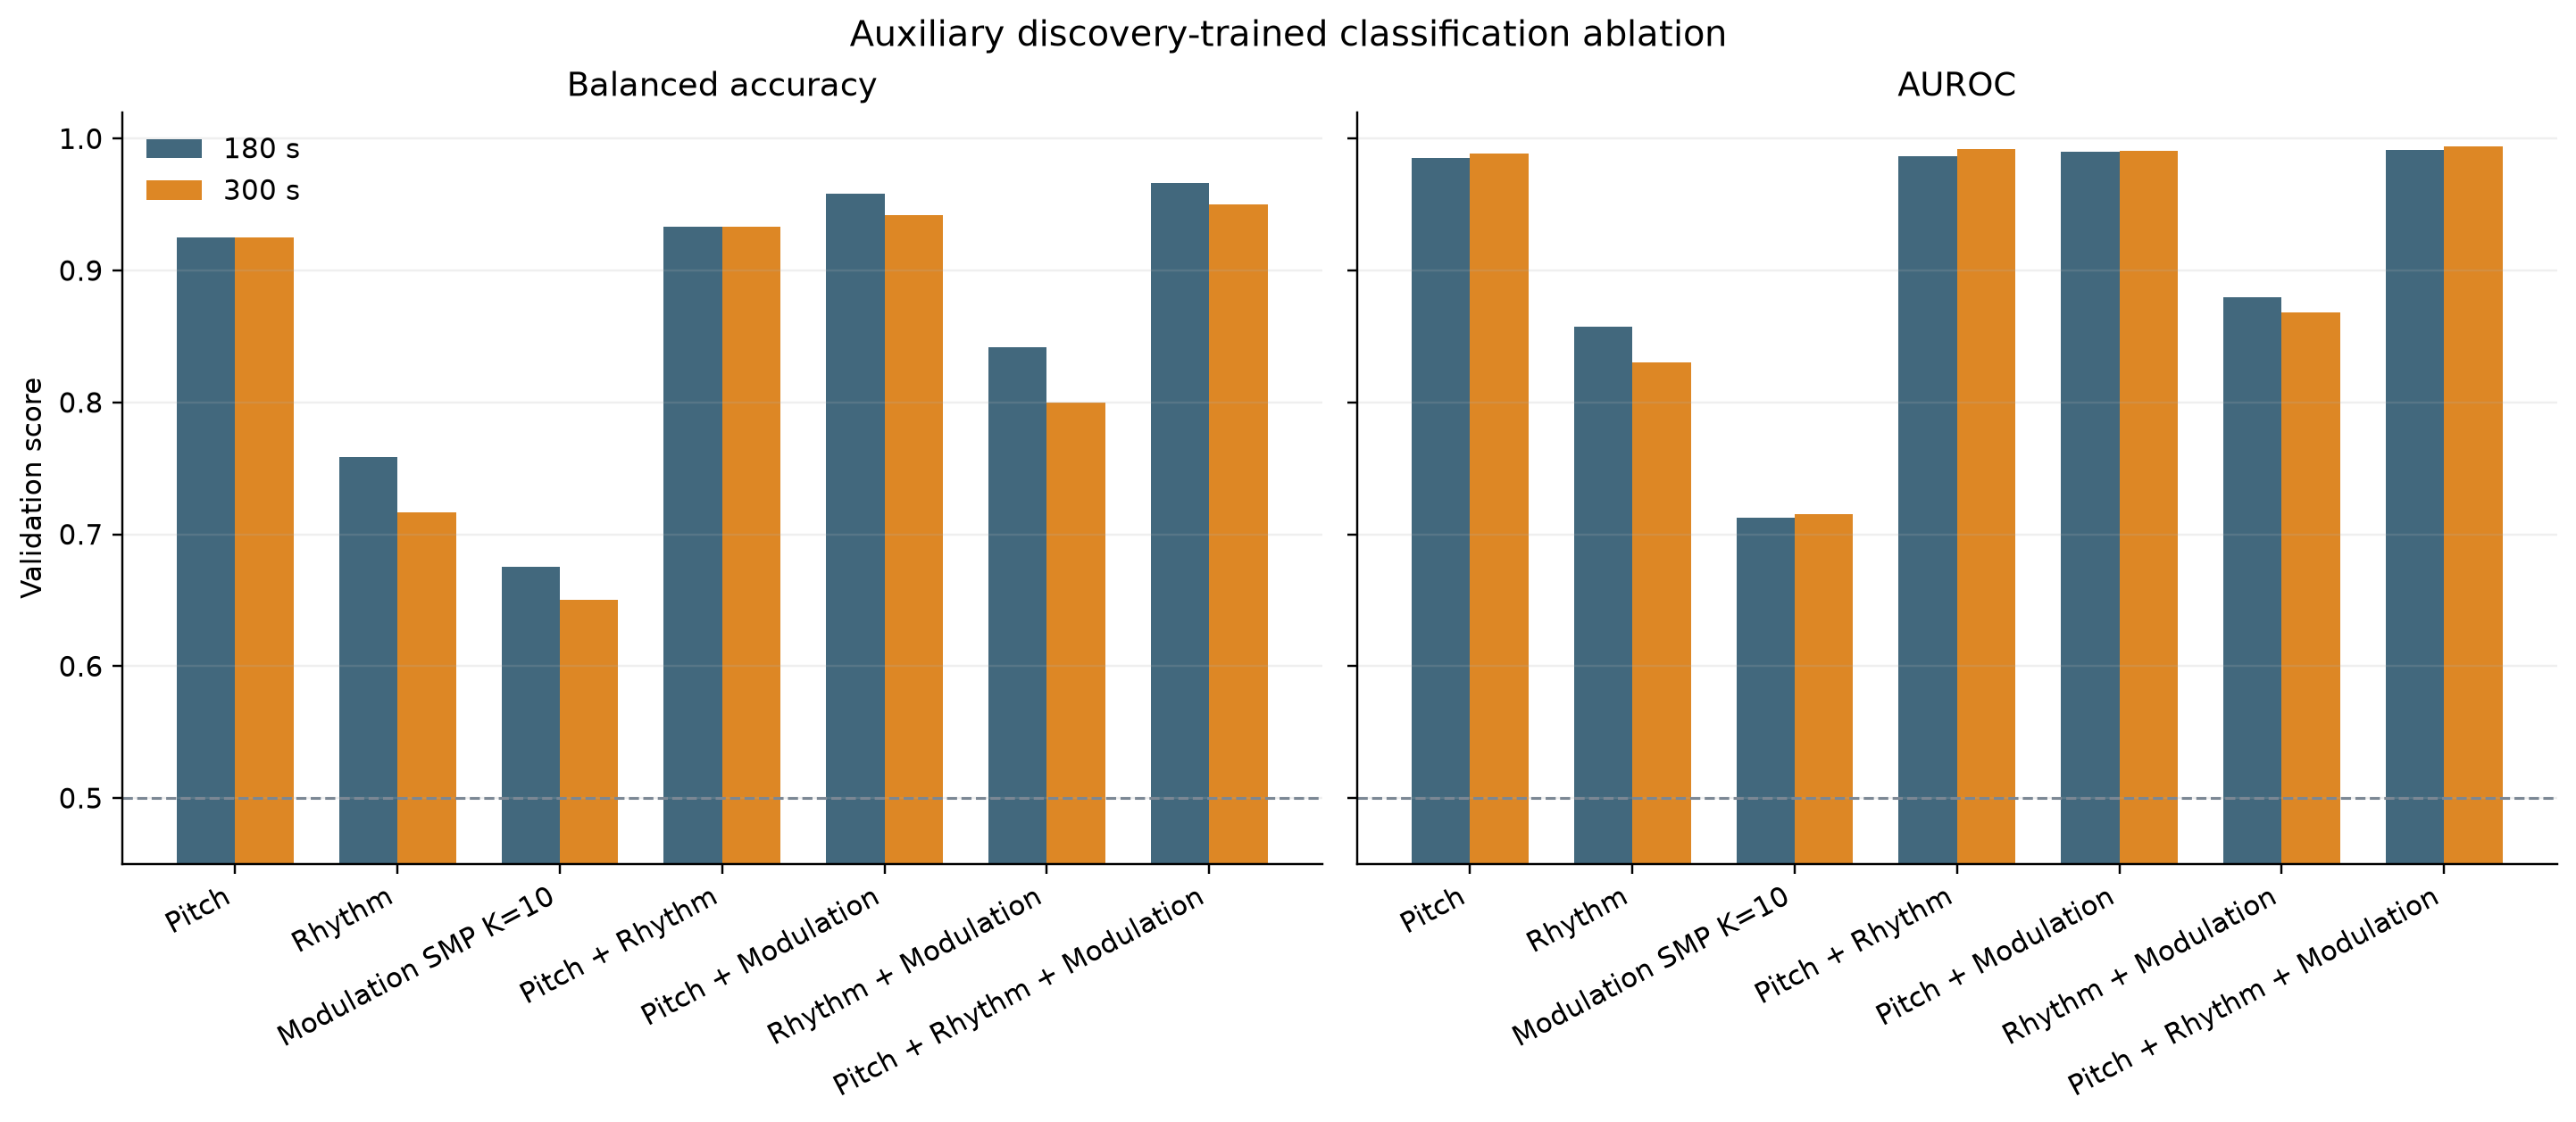
\includegraphics[width=\textwidth]{fig/local_smp_k10_classification_ablation.png}
    \caption{由 discovery/180s 冻结的辅助分类消融结果。分类结果用于补充距离几何检验，不替代 PERMANOVA 或配对增量检验。}
    \label{fig:local_fusion_classification}
\end{figure}

\paragraph{综合判断与证据边界}
局部三视角等权融合保留了稳定的组间可分性，并在辅助逐曲分类上优于音高单视角；但它没有提高相对最佳单视角的 pseudo-$F$，且留一视角检验只确认了音高的正向几何增量。节奏和调制具有条件非冗余与独立解释价值，却尚无证据表明它们在当前等权距离中提供稳定的增量分离。因此，\textbf{本文将音高视为局部指纹的主要分离块，将节奏与调制保留为互补解释块，而不宣称三视角融合在整体上优于最佳单视角}。

\subsection{拓扑指纹冻结}
\label{sec:frozen_topology_fingerprint}

前述分析产生两个用途不同、不能相互替代的版本化对象。首先，原分析协议冻结的是
$18$ 维 Pitch--Phase 观察性表示：它保留 $16$ 维 Pitch 白化坐标以及 Acoustic、Chroma
phase 的两个 \texttt{loop\_score}，用于复现本章既有的距离、增量和分类分析；其版本号为
\nolinkurl{focus_path_homology_fingerprint_v2}。
由于该对象先于后续生成目标简化而冻结，本文保留其身份与证据边界，不用事后选择的
三个指标改写原确认性分析。

其次，多尺度结果显示，Pitch 是当前局部融合中唯一具有稳定正向几何增量的视角，
而跨周期相位与联合表示没有稳定优于最佳 Pitch 单块。

为降低潜空间代理的样本复杂度，生成侧另行冻结三维局部指纹
\nolinkurl{focus_pitch3_fingerprint_v1}，记为
\begin{equation}
\Phi_{\mathrm{P3}}(x)=
\left[z_{H_0}(x),z_{\mathrm{self}}(x),z_{\mathrm{rec}}(x)\right]
\in\mathbb R^3.
\label{eq:frozen_pitch3_fingerprint}
\end{equation}
它只服务于精确教师、代理训练和后续生成控制。由于指标选择发生在查看 validation
结果之后，该对象明确登记为 \textit{post-validation downstream refreeze}，不能产生
新的确认性组间结论。

\begin{table}[htbp]
\centering
\caption{Pitch-3 下游拓扑指纹的冻结组成与选择依据}
\label{tab:frozen_fingerprint}
\setlength{\tabcolsep}{3pt}
\begin{tabular}{p{0.29\linewidth}p{0.25\linewidth}crr}
\toprule
原始指标 & 结构含义 & Focus 方向 & 180s BH-FDR $q$ & 180/300s $\rho$ \\
\midrule
\texttt{h0\_observed\_persistence} & 局部连通与状态覆盖 & 较低 & $8.94\times10^{-19}$ & 0.953 \\
\texttt{self\_transition\_ratio} & 局部稳定与停留 & 较高 & $3.97\times10^{-16}$ & 0.979 \\
\texttt{directed\_recurrence} & 有向重复结构 & 较高 & $1.16\times10^{-16}$ & 0.983 \\
\bottomrule
\end{tabular}
\end{table}

三个指标分别覆盖连通性、停留性和有向复现，避免仅保留节点数、边数等高度依赖图规模
且机制重叠的计数特征。它们在原预设 Pitch 检验族中均通过 validation/180s 的
BH-FDR，并在同曲 validation/300s 保持方向和较高配对 Spearman 相关；这些数值用于
记录选择依据，不把事后筛选重新表述为预注册验证。三维逻辑回归在 validation/180s
的 balanced accuracy 为 $0.942$、AUROC 为 $0.980$，在 300s 敏感性分析中的对应值为
$0.942$ 和 $0.988$；这些结果说明压缩后仍保留主要判别信息，但不等于生成可控性证据。

除表~\ref{tab:frozen_fingerprint} 的指标顺序外，以下字段一并冻结：
\begin{enumerate}
  \item 状态码本与三个原始描述子沿用 Pitch 分支的既有定义；标准化只使用
  discovery/180s，中心取中位数，尺度优先取归一化 IQR，并以归一化 MAD 和标准差
  依次回退；
  \item 坐标顺序固定为 $H_0$ observed persistence、self-transition ratio、
  directed recurrence，三维距离及带外损失权重均为 $1/3$；
  \item Focus 目标带只由 discovery/180s Focus 样本各坐标的第 $10$--$90$
  百分位数确定；具体中心、尺度和目标带见表~\ref{tab:pitch3_contract}；
  \item validation/180s 记录主要统计支持，validation/300s 仅作同曲时长敏感性；
  holdout 不参与三指标选择、变换拟合、目标带设定或阈值调整；
  \item 指纹 JSON、逐曲分数、配置、代码和来源表均以 SHA-256 绑定。任何特征替换、
  顺序变化、重新加权或目标带修改都必须建立新版本。
\end{enumerate}

因此，本文的观察性结论仍由原 $18$ 维分析合同承载，而生成方法使用更小的
$\Phi_{\mathrm{P3}}$。两者都不是注意力、疗效或音乐质量的因果量表；Pitch-3 指纹本身
也不授权采样期校正，只有代理在独立资格检验中满足预测、校准、OOD 与解码后精确方向
门槛后，corrector 才能由关闭状态转为候选启用。

\section{ACE-Step 拓扑引导音乐生成}

\subsection{研究边界与方法概览}

本文进一步考察如何在不重新训练基础生成模型的前提下，将局部 Pitch Path Homology 用作 ACE-Step 1.5 XL-Turbo 的推理期控制信号\cite{gong2026}。与直接在波形域计算控制损失并反向传播穿过 VAE 解码器的方法相比，潜空间控制头可以显著降低单次梯度计算的显存和时间开销；Novack 等人提出的 Latent-Control Head（LatCH）与 selective TFG 已验证了这种``潜变量到控制量''路线的可行性\cite{novack2026}。本文沿用其低资源思想，但控制对象不是逐帧强度、音高类别或节拍曲线，而是整段音乐的三个全局局部拓扑坐标。

方法仍遵循``精确教师--可微代理--精确复核''闭环：精确 Pitch PH 从每个独立解码的轨迹快照生成三维标签；轻量潜空间拓扑控制头（Latent Topology Control Head for Pitch-3，LTCH-P3）学习从预测干净潜变量到该标签的可微映射；只有在未见 prompt、seed family 与生成轨迹上通过预测、校准、OOD 和解码后方向一致性门槛，代理梯度才允许在少数采样步骤中启用。最终音频仍由精确教师、音质指标与 prompt 一致性共同裁决。

\subsection{三维精确拓扑教师}

令 $f(x)\in\mathbb R^3$ 表示从音频 $x$ 的完整 Pitch 图描述子中选出的三个互补指标：
\begin{equation}
f(x)=\left[
f_{H_0}(x),\ f_{\mathrm{self}}(x),\ f_{\mathrm{rec}}(x)
\right],
\end{equation}
其中 $f_{H_0}$ 为 \texttt{h0\_observed\_persistence}，刻画局部连通与状态覆盖；$f_{\mathrm{self}}$ 为 \texttt{self\_transition\_ratio}，刻画局部停留；$f_{\mathrm{rec}}$ 为 \texttt{directed\_recurrence}，刻画有向重复。三项均在 validation/180s 通过原预设 Pitch 检验族的 BH-FDR，并在同曲 validation/300s 中保持方向和较高配对相关；选择规则强调统计支持、跨时长稳定和机制互补，而不是简单截取旧白化坐标。

所有变换只使用 discovery/180s 拟合。设第 $j$ 项的 discovery 中位数为 $m_j$，稳健尺度为 $s_j$，则冻结坐标为
\begin{equation}
z_j(x)=\frac{f_j(x)-m_j}{s_j},\qquad
z(x)=[z_{H_0},z_{\mathrm{self}},z_{\mathrm{rec}}]\in\mathbb R^3.
\label{eq:pitch3_coordinate}
\end{equation}
冻结参数和 discovery Focus 的目标带列于表~\ref{tab:pitch3_contract}。

\begin{table}[htbp]
\centering
\caption{Pitch-3 精确教师的冻结标准化与目标带}
\label{tab:pitch3_contract}
\begin{tabular}{lrrr}
\toprule
坐标 & 中心 $m_j$ & 尺度 $s_j$ & Focus 目标带 $[l_j,u_j]$ \\
\midrule
$H_0$ observed persistence & $4.2000$ & $2.3629$ & $[-1.265,-0.042]$ \\
self-transition ratio      & $0.4600$ & $0.2800$ & $[0.041,1.184]$ \\
directed recurrence        & $0.05685$ & $0.08077$ & $[0.117,3.133]$ \\
\bottomrule
\end{tabular}
\end{table}

目标带由 discovery Focus 各坐标的第 $10$--$90$ 百分位数确定。三个坐标等权，精确带外损失定义为
\begin{equation}
L_{\mathrm{band}}(z)=\frac{1}{3}\sum_{j=1}^{3}
\left\{
[\max(l_j-z_j,0)]^2+[\max(z_j-u_j,0)]^2
\right\}.
\label{eq:pitch3_band_loss}
\end{equation}
样本进入经验支持区间后，该坐标的梯度归零，因而控制目标是回到 Focus 参考分布邻域，而不是无限降低 $H_0$ 或无限提高重复率。另在 discovery/180s 上冻结三维 L2 逻辑回归
\begin{equation}
S_F(x)=w^\top z(x)+b,
\end{equation}
作为联合方向的辅助读出；由于三个坐标仍有相关性，$S_F$ 不作为唯一引导能量，避免模型利用线性分类边界中的相关性捷径。

\subsection{预测干净潜变量与时间条件}

ACE-Step XL-Turbo 的声学潜变量记为 $x_t\in\mathbb R^{B\times T\times64}$。LTCH-P3 不只读取最终潜变量，而读取每个被标注采样步自身的预测干净潜变量。对当前 flow-matching 参数化，定义
\begin{equation}
\hat{x}_{0|t}=x_t-t v_t,
\label{eq:pred_clean_latent}
\end{equation}
其中 $v_t$ 是基础模型在噪声时间 $t$ 的速度预测。连续时间 $t$ 与离散 step id 分别作多频 Fourier 编码，再经两层 MLP 得到 $128$ 维条件向量
\begin{equation}
e_t=\operatorname{MLP}(\operatorname{Fourier}(t,\mathrm{step}))
\in\mathbb R^{128}.
\end{equation}
该条件向量被投影为通道尺度和偏移，对时序特征执行
\begin{equation}
h'_i=h_i\odot[1+\gamma(e_t)]+\beta(e_t),
\end{equation}
使网络能够区分同一潜结构在不同去噪阶段上的可信度。

\subsection{LTCH-P3 网络结构}

LTCH-P3 是面向整段 $180$ 秒音频的全局控制头，不输出逐帧控制曲线。其计算流程见图~\ref{fig:pitch3_architecture}。

\begin{figure}[htbp]
\centering
\resizebox{\textwidth}{!}{%
\begin{tikzpicture}[
  >={Stealth[length=2mm]},
  box/.style={draw, rounded corners, align=center, minimum height=11mm,
              text width=29mm, font=\small, inner sep=2pt},
  arr/.style={->, thick},
]
\definecolor{cinput}{HTML}{DCE9F7}
\definecolor{ccond}{HTML}{FCE5CD}
\definecolor{cmodel}{HTML}{E2D5F0}
\definecolor{cpool}{HTML}{D9EAD3}
\definecolor{cout}{HTML}{FFF2B3}
\node[box,fill=cinput] (a) at (0,0) {$\hat{x}_{0|t}$\\$[B,T,64]$};
\node[box,fill=cmodel] (b) at (3.8,0) {逐帧 LayerNorm\\Linear $64\to128$};
\node[box,fill=cmodel] (c) at (7.6,0) {Depthwise Conv1d\\$k=9,s=4$};
\node[box,fill=ccond] (d) at (7.6,2.1) {$t$ 与 step\\Fourier--MLP $128$};
\node[box,fill=cmodel] (e) at (11.4,0) {FiLM + 位置编码\\$3\times$ Transformer};
\node[box,fill=cpool] (f) at (15.2,0) {Attention/Mean/Std\\pool $384$ + $e_t$};
\node[box,fill=cpool] (g) at (19.0,0) {Fusion MLP\\$512\to256\to128$};
\node[box,fill=cout] (h) at (22.8,0) {$\hat\mu_z[3]$, $\log\hat\sigma_z^2[3]$\\OOD[1], Focus logit[1]};
\draw[arr] (a)--(b);
\draw[arr] (b)--(c);
\draw[arr] (c)--(e);
\draw[arr] (d)--(e);
\draw[arr] (d.east) to[bend left=18] (f.north);
\draw[arr] (e)--(f);
\draw[arr] (f)--(g);
\draw[arr] (g)--(h);
\end{tikzpicture}%
}
\caption{LTCH-P3 的全局三维潜空间拓扑代理结构。}
\label{fig:pitch3_architecture}
\end{figure}

首先对输入逐帧执行 LayerNorm 和 $64\to128$ 线性投影。随后使用 depthwise \texttt{Conv1d}（kernel $9$、stride $4$、padding $4$）将长度从 $T$ 降到约 $\lceil T/4\rceil$；卷积只作逐通道时间聚合，通道混合由前置线性层完成。相对于直接在全长序列上自注意力，该操作将注意力矩阵的渐近开销降至约原来的 $1/16$。

下采样序列加入正弦绝对位置编码，并经三个 pre-norm Transformer encoder block。每层使用 $d_{\mathrm{model}}=128$、$4$ 个注意力头、FFN 宽度 $512$、GELU 和 dropout $0.1$。本文未直接复制 LatCH 的 RoPE，而保留更简单的固定位置编码；该选择应在真实长序列训练后再决定是否需要位置编码消融。

Transformer 输出经掩码 attention pooling、均值 pooling 和标准差 pooling，得到 $128\times3=384$ 维全局统计；与 $128$ 维时间条件拼接为 $512$ 维，经 $512\to256\to128$ 的 SiLU MLP 得到共享表征。按当前层配置计算，模型约含 $0.87$M 个可训练参数，低于 Novack 等人约 $7$M 参数的 LatCH 规模\cite{novack2026}。这种压缩主要来自三维全局目标，而非时间对齐的高维控制序列。

输出包括三维坐标均值、三维对数方差和一个 OOD logit：
\begin{equation}
g_\phi(\hat{x}_{0|t},t)
=\left(\hat\mu_z,\log\hat\sigma_z^2,u_{\mathrm{OOD}}\right).
\end{equation}
对数方差限制在 $[-8,4]$。冻结 Focus logit 不设置独立自由分类头，而由
\begin{equation}
\hat S_F=w^\top\hat\mu_z+b
\end{equation}
确定性计算，从而保证联合读出与预测坐标一致。对数方差表示单模型 aleatoric uncertainty；其校准和 OOD 阈值必须在独立 calibration 分区完成，当前不能直接解释为有效置信区间。

\subsection{教师标签、数据构造与防泄漏}

每个训练样本为 $(\hat{x}_{0|t},t,z,S_F,y_{\mathrm{OOD}})$。在无引导生成轨迹中保存第 $4$、$5$、$6$ 步及最终步的 $(x_t,v_t,t)$，按式~\eqref{eq:pred_clean_latent} 构造各自的 $\hat{x}_{0|t}$，分别经 VAE 解码，再独立运行 exact Pitch PH。不得把最终音频标签复制到中间步骤，否则网络会学习错误的时间不变映射。

正式 prompt 清单包含 $512$ 个变体，按 prompt family 固定为 train/development/calibration/qualification 的 $320/64/64/64$ 划分；每个 prompt 计划生成 $4$ 个确定性 seed，共 $2048$ 条轨迹和最多 $8192$ 个常规快照。安全/OOD 样本包括静音、削波、极低动态、机械短循环、过度平滑和异常潜变量，但不得通过改变资格门槛来迁就 OOD 失败。

数据清单强制校验指纹 SHA-256、三维坐标顺序、latent SHA-256 和逐快照标签来源。同一 prompt、同一 prompt family、同一轨迹及其全部 seed/快照必须位于同一分区。论文的 validation 与已开启 holdout 只承担拓扑证据和历史兼容性说明，不用于 LTCH-P3 的架构选择、损失调权、early stopping 或阈值校准。

\subsection{损失函数与训练配置}

只有 ID 样本参与坐标、异方差和 Focus 读出回归，全部样本参与 OOD 分类。坐标损失为
\begin{equation}
L_{\mathrm{coord}}=
\frac{1}{3}\sum_{j=1}^{3}
\operatorname{SmoothL1}(\hat\mu_j-z_j).
\end{equation}
令 $s_j=\log\hat\sigma_j^2$，异方差负对数似然为
\begin{equation}
L_{\mathrm{NLL}}=
\frac{1}{6}\sum_{j=1}^{3}
\left[e^{-s_j}(\hat\mu_j-z_j)^2+s_j\right].
\end{equation}
辅助读出损失为 $L_{\mathrm{Focus}}=\operatorname{SmoothL1}(\hat S_F-S_F)$，安全损失为带类别权重的 $L_{\mathrm{OOD}}=\operatorname{BCEWithLogits}(u_{\mathrm{OOD}},y_{\mathrm{OOD}})$。当前代码合同冻结总损失
\begin{equation}
L=L_{\mathrm{coord}}+0.25L_{\mathrm{NLL}}
+0.25L_{\mathrm{Focus}}+0.1L_{\mathrm{OOD}}.
\label{eq:pitch3_total_loss}
\end{equation}

训练使用 AdamW，初始学习率 $2\times10^{-4}$、weight decay $10^{-4}$、micro-batch size $8$、最大 $40$ epochs；至少训练 $8$ epochs 后，若 development 总损失连续 $7$ epochs 无改善则 early stop；全局梯度范数裁剪为 $1.0$。支持 bf16 前向，但损失和检查点统计保持 fp32。训练阶段只读取预计算 latent 与精确标签，不加载 ACE-Step DiT 或 VAE。每个 checkpoint 原子写入并绑定指纹、训练配置与数据清单哈希，且默认写入 \texttt{guidance\_promotion\_eligible=false} 和 \texttt{production\_authorization=false}。

\subsection{选择性采样校正与安全回退}

通过资格检验后，LTCH-P3 可作为 selective latent guidance 的控制头。在选定采样步，将基础模型计算从梯度图中分离，只对预测干净潜变量开启梯度：
\begin{equation}
\tilde{x}_{0|t}=\operatorname{stopgrad}(x_t-tv_t),
\qquad \tilde{x}_{0|t}.\mathrm{requires\_grad}=\mathrm{True}.
\end{equation}
代理能量采用式~\eqref{eq:pitch3_band_loss} 在预测均值上的版本：
\begin{equation}
\widehat{\mathcal E}_t=
L_{\mathrm{band}}(\hat\mu_z(\tilde{x}_{0|t},t)),
\qquad
g_t=\nabla_{\tilde{x}_{0|t}}\widehat{\mathcal E}_t.
\label{eq:pitch3_guidance}
\end{equation}
若 OOD 概率、预测方差、NaN/Inf、哈希不一致或掩码检查任一超阈，则该样本必须 no-op。有效梯度经时间低通和相对 RMS clip 后，才可映射到下一潜变量状态。初始设计仍只考察第 $4$--$6$ 步，避免高噪声早期和直接输出端；步间权重与 RMS 半径只能在 development 上从预设候选中选择一次。

需要强调的是，当前仓库已经实现三维精确教师、LTCH-P3、哈希标签清单和训练入口，但尚未实现并授权新的采样器 corrector。上述更新式是待资格检验的推理协议，不是已取得的生成结果。

\subsection{资格检验、最终评价与当前状态}

LTCH-P3 只有在未见 prompt、seed family 和轨迹上同时满足以下条件，才允许进入采样器：Focus logit Spearman $\rho\geq0.70$；三个坐标各自及其中位数 Spearman 均不低于 $0.50$；三维目标带距离 Spearman 不低于 $0.50$；exact 高/低四分位排序准确率不低于 $0.65$；$90\%$ 预测区间覆盖率位于 $0.85$--$0.95$；校正步骤的 ID 接受率不低于 $0.95$；OOD AUROC 与 sensitivity 均不低于 $0.80$；代理优化后解码音频的 exact 改善方向一致率不低于 $0.65$。任一坐标、OOD 或解码后方向门槛失败，都不能由总体 Focus logit 掩盖。

最终确认实验继续采用未参与开发的 $32$ 个 prompts、每个 prompt $8$ 个 seeds，形成 $256$ 对 baseline/guided 配对和 $512$ 首 $180$ 秒音频。主要终点为
\begin{equation}
\Delta_i=L_{\mathrm{band}}^{\mathrm{guided}}(i)
-L_{\mathrm{band}}^{\mathrm{base}}(i),
\end{equation}
其中负值表示更接近冻结三维目标带。报告中位差、Hodges--Lehmann 位移、按 prompt 聚类的 bootstrap $95\%$ 置信区间及目标带命中率；同时执行 prompt 一致性、响度、true peak、削波、静音、频谱异常、机械短循环、过度平滑、多样性、运行时间和显存的预设非劣检验。若能完成合规审批，再把盲听作为补充终点，而不以主观结果替代精确拓扑和技术质量门槛。

\begin{tcolorbox}[colback=yellow!20,colframe=yellow!60!black,boxrule=0.5pt,arc=6pt,left=6pt,right=6pt,top=4pt,bottom=4pt]
\textbf{当前证据状态：}三维指纹已由 discovery/180s 稳健变换冻结，并在现有 $1200$ 个 $180/300$ 秒片段上完成确定性数值重建；代理网络、训练器和标签清单已通过本地静态及非 Torch 测试。由于本机没有 PyTorch/CUDA，真实 ACE-Step 轨迹收集、LTCH-P3 训练、OOD 校准、解码后方向一致性和最终 baseline/guided 评价均尚未执行。因此，本节只报告已实现的方法与预设门槛，采样期 corrector 继续保持关闭。
\end{tcolorbox}

\iffalse % Legacy 18-D generation section retained as an inactive audit trail.

本文的目的之一是将 focus music 的拓扑特征用于音乐生成。传统路线会选择训练一个新的音乐生成模型，并将拓扑特征作为损失函数嵌入训练循环。然而，高质量音乐生成模型的训练需要大量版权敏感的音频数据，并且对 GPU 算力要求高，因此本研究将工程核心从``更新模型参数 $\theta$''转向``控制推理期潜变量 $z_t$''。

本研究选用 ACE-Step 1.5 XL-Turbo 作为基础骨干网络，在其逆向扩散采样的关键时间步，对当前音频潜变量施加来自冻结 Path Homology 指纹的拓扑能量梯度。这样既保留了预训练模型的音乐生成能力，又让生成过程受到可解释的代数拓扑约束。

\subsection{方法思想与总体框架}

由于精确 Path Homology（exact PH） 包含一系列``非光滑操作''，这些操作几乎处处梯度为 $0$ 或未定义，无法通过链式法则传递有效梯度。因此我们训练了潜空间拓扑代理网络（Latent Topology Surrogate Network，LTSN）用于提供近似的、可导的评分，用它来反向传播梯度。它学习的目标就是去模仿 exact PH 的输出，同时保持整个计算图可微。

整个方法的核心是一个``精确教师--可微代理--精确复核''闭环：
exact PH 负责构造训练标签、执行同 prompt 候选重排并对最终音频作出裁决；LTSN 仅学习从中间预测干净潜变量到冻结指纹的可微近似；采样器只在 LTSN 通过独立资格检验后施加幅度受限的中段校正。生成结果在解码后仍须由 exact PH、音质指标和 prompt 一致性共同复核。整体流程如图~\ref{fig:acestep_pipeline} 所示。

\begin{figure}[htbp]
\centering
\resizebox{\textwidth}{!}{%
\begin{tikzpicture}[
    >={Stealth[length=2.2mm]},
    box/.style={draw, rounded corners, align=center,
                minimum height=12mm, text width=24mm,
                font=\small, fill=white, inner sep=2pt},
    decision/.style={draw, diamond, align=center, aspect=2.4,
                     text width=20mm, font=\small, fill=white, inner sep=1pt},
    arr/.style={->, thick},
    darr/.style={->, thick, dashed},
    lbl/.style={font=\scriptsize, fill=white, inner sep=1pt},
]
% ---- 节点背景色：按角色分组 ----
% 输入/数据：浅蓝；精确教师：浅红；标签产物：浅橙；
% 代理模型：浅紫；决策检验：浅黄；校正/解码：浅绿；
% 终止接受：浅青；回退层级：浅灰
\definecolor{cin}{HTML}{DCE9F7}      % 输入/候选
\definecolor{cteacher}{HTML}{F8D7DA}  % 精确教师
\definecolor{clabel}{HTML}{FCE5CD}    % 训练标签
\definecolor{cproxy}{HTML}{E2D5F0}    % 可微代理
\definecolor{cdecision}{HTML}{FFF2B3} % 决策检验
\definecolor{cact}{HTML}{D9EAD3}     % 校正/解码动作
\definecolor{caccept}{HTML}{D0E8E0}  % 接受结果
\definecolor{cback}{HTML}{EAEAEA}     % 回退层级
% ---- 主流水线（上排 L->R，下排 R->L）----
\node[box, fill=cin]        (A) at (0, 0)   {ACE-Step 同 prompt\\候选音频与中间潜变量};
\node[box, fill=cteacher]   (B) at (4, 0)   {精确教师\\Exact PH};
\node[box, fill=clabel]     (C) at (8, 0)   {训练标签\\18 维冻结指纹与 Focus logit};
\node[box, fill=cproxy]     (E) at (12, 0)  {可微代理 LTSN\\预测拓扑坐标与不确定度};
\node[decision, fill=cdecision] (F) at (12, -3) {独立资格检验};
\node[box, fill=cact]       (G) at (8, -3)  {中段弱校正};
\node[box, fill=cact]       (H) at (4, -3)  {最终音频解码};
\node[decision, fill=cdecision] (I) at (4, -6)  {精确复核};
\node[box, fill=caccept]    (J) at (0, -6)  {接受生成结果};
% ---- 上方分支：候选重排与回退层级 ----
% \node[box] (D) at (3.4, 3.4)    {候选重排\\Exact best-of-$N$};
\node[box, fill=cback]      (K) at (12, -6) {停止或回退至\\exact reranking};

% ---- 实线箭头 ----
\draw[arr] (A) -- (B);
\draw[arr] (B) -- node[lbl, above]{逐快照精确标注} (C);
% \draw[arr] (B) -- node[lbl, right]{同 prompt 精确评分} (D);
\draw[arr] (C) -- node[lbl, above]{监督训练} (E);
\draw[arr] (E) -- (F);
\draw[arr] (F) -- node[lbl, above]{通过} (G);
\draw[arr] (G) -- (H);
\draw[arr] (H) -- (I);
\draw[arr] (I) -- node[lbl, above]{全部通过} (J);
\draw[arr] (F) -- node[lbl, sloped, above]{未通过} (K);
\draw[arr] (I) -- node[lbl, sloped, above, align=center]{代理偏离或质量退化} (K);
\draw[arr] (A) to
    node[lbl, below, align=center]{预测干净潜变量 $\hat{x}_0$} (G);

% ---- 虚线箭头：冻结规则与回退 ----
\draw[darr] (B) to[bend right=50]
    node[lbl, sloped, below]{冻结评分规则} (I);
% \draw[darr] (K) -- node[lbl, above]{保留可靠层级} (D);
\end{tikzpicture}%
}
\caption{精确教师--可微代理--精确复核闭环。}
\label{fig:acestep_pipeline}
\end{figure}

整个生成侧按照以下门控顺序推进：首先重建并冻结 $18$ 维 exact scorer；随后在不改变生成结果的 shadow mode 中保存轨迹；再检验同 prompt 候选池中是否存在可由 exact scorer 稳定识别的差异；只有 exact reranking 有效，才训练并检验 LTSN；最后开发弱梯度 corrector。该顺序将``候选空间是否可辨识''与``代理能否忠实逼近''置于采样控制之前，避免用复杂引导掩盖目标本身不可识别的问题。

\subsection{冻结目标与目标带损失}

令生成音频为 $x$，其冻结指纹为
\begin{equation}
z(x)=\Phi_{\mathrm{PH}}(x)
=\frac{1}{\sqrt{2}}\left[L(x)\Vert P(x)\right]\in\mathbb{R}^{18},
\end{equation}
其中 $L=Z_{\mathrm{Pitch}}\in\mathbb{R}^{16}$，
$P=\frac{1}{\sqrt{2}}[Z_{\mathrm{Acoustic}}\Vert
Z_{\mathrm{Chroma}}]\in\mathbb{R}^{2}$。

在 discovery/180s 数据上，用冻结的 L2 逻辑回归将指纹读出为 Focus 判别 logit：
\begin{equation}
S_F(x)=w^{\top}z(x)+b,\qquad p_F(x)=\sigma(S_F(x)).
\end{equation}
为防止引导无限抬高 logit，本文从 discovery Focus logit 的预设低分位数确定目标带下界 $\tau_F$，并定义
\begin{equation}
L_{\mathrm{PH}}(x)=\left[\max\left(0,\tau_F-S_F(x)\right)\right]^2.
\label{eq:focus_band_loss}
\end{equation}
样本进入目标带后梯度归零。因此，控制目标是进入经验支持的 Focus 分布邻域，而不是把任一拓扑坐标推向极端。

\subsection{输入与时间条件}

ACE-Step 1.5 XL-Turbo 的声学潜变量为 $64$ 维，声学潜变量记为 $x_t\in\mathbb{R}^{B\times T\times64}$。180s 音频在约 25Hz 的潜时间分辨率下对应 $T= 180 \times 25 = 4500$。LTSN 的输入是每个采样步自身的 $\hat{x}_0$，而非仅使用最终 \texttt{pred\_latents}。输入必须由真实的 $x_t$、速度 $v_t$ 和噪声时间 $t$ 构造 $\hat x_0$。对 flow matching 模型，相应的预测干净潜变量为
\begin{equation}
\hat{x}_0=x_t-tv_t.
\label{eq:pred_clean_latent}
\end{equation}

\begin{figure}[htbp]
    \centering
    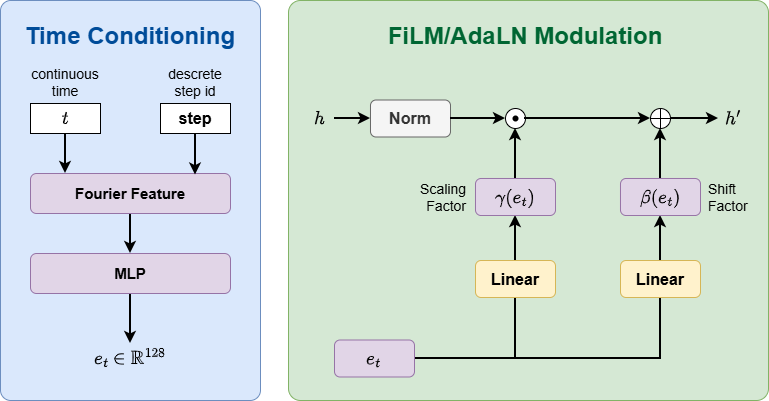
\includegraphics[width=0.8\textwidth]{fig/time_conditioning.png}
    \caption{LTSN 时间条件模块。}
    \label{fig:time_conditioning}
\end{figure}

相同幅度的潜变量误差在不同噪声时间上含义不同，因此将连续时间 $t$ 与离散 step id 经 Fourier 特征和两层 MLP 编码为 $128$ 维条件向量：
\begin{equation}
e_t=\operatorname{MLP}(\operatorname{Fourier}(t,\text{step}))
\in\mathbb R^{128},
\end{equation}
并通过 FiLM/AdaLN 调制时序残差块：
\begin{equation}
\operatorname{FiLM}(h,e_t)=\gamma(e_t)\odot\operatorname{Norm}(h)+\beta(e_t).
\end{equation}

\subsection{潜空间拓扑代理网络（LTSN）}

\begin{figure}[htbp]
    \centering
    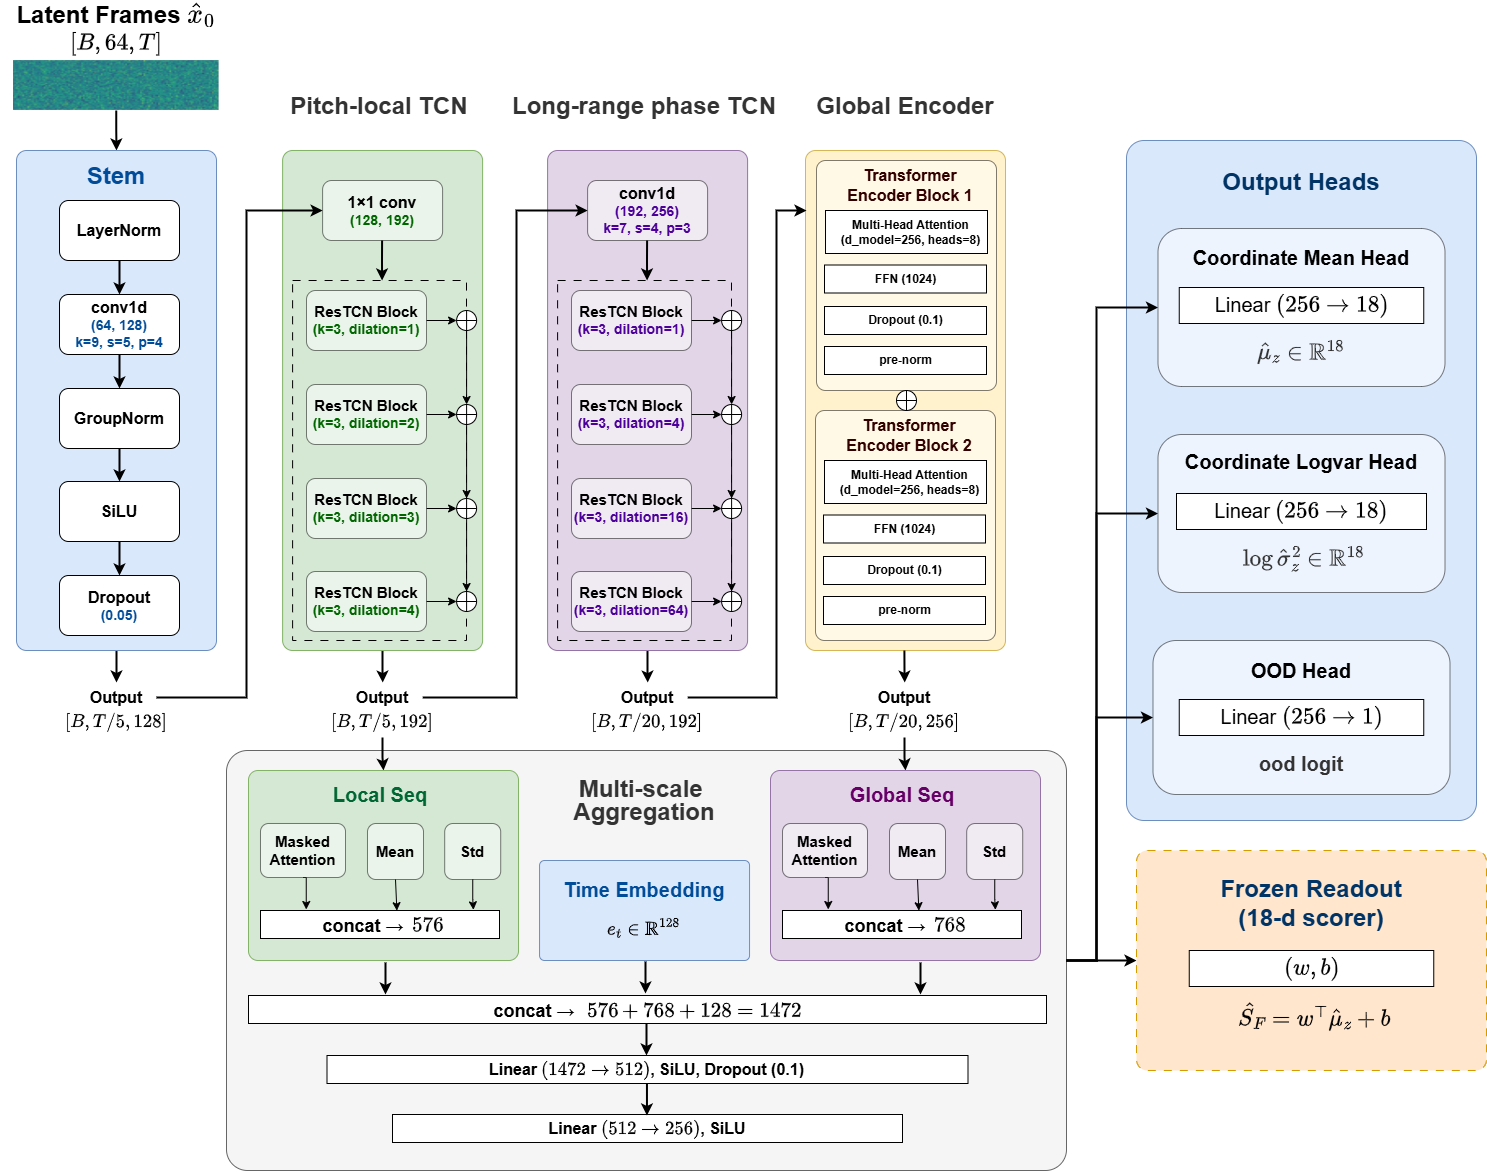
\includegraphics[width=\textwidth]{fig/architecture.png}
    \caption{LTSN 架构图。}
    \label{fig:ltsn_architecture}
\end{figure}

\subsubsection{Stem}

Stem 的结构可以概括为：
\[\hat{x}_0 \to \texttt{LayerNorm} \to \texttt{Conv1d} \to \texttt{GroupNorm} \to \texttt{SiLU} \to \texttt{Dropout(0.05)}\]
它主要完成两个任务：
\begin{itemize}
    \item 将 $64$ 维声学潜变量扩展到 $128$ 维特征；
    \item 将 25 Hz 的潜变量下采样到 5 Hz。
\end{itemize}
\verb|Conv1d| 卷积参数为 \verb|(64, 128, kernel=9, stride=5, padding=4)|。\verb|kernel = 9|，在 25 Hz 下对应：$9/25=0.36 \text{s}=360 \text{ms}$，\verb|stride = 5|，对应：$5/25=0.2s=200ms$。所以每个输出帧大约覆盖 $360$ ms 的输入上下文，输出帧之间间隔 $200$  ms。最终输出特征为 $[B, T/5, 128]$。

\subsubsection{Pitch-local TCN}

Stem 后用 $1 \times 1$ 卷积投影到 $192$ 通道，再串联四个残差 TCN 块：

\begin{table}[htbp]
\centering
\caption{Pitch-local TCN 残差块配置}
\begin{tabular}{lrrrr}
\toprule
block & \texttt{kernel} & \texttt{dilation} & 通道 & 作用  \\
\midrule
\#1     & $3$      & $1$        & $192$  & 局部相邻 token    \\
\#2     & $3$      & $2$        & $192$  & 短时谐波状态变化  \\
\#3     & $3$      & $4$        & $192$  & 数秒局部组织     \\
\#4     & $3$      & $8$        & $192$  & 较长局部上下文   \\
\bottomrule
\end{tabular}
\end{table}

每个块的内部结构为：
\begin{figure}[htbp]
    \centering
    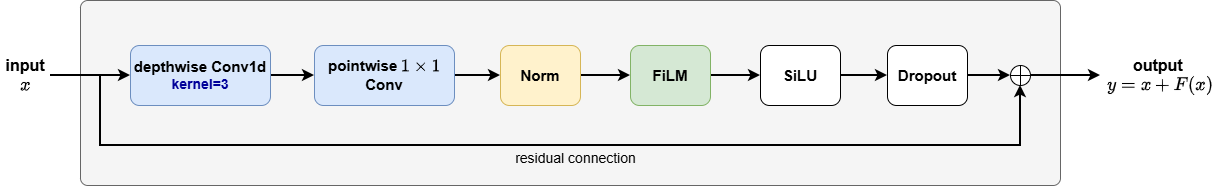
\includegraphics[width=\textwidth]{fig/tcn_block.png}
    \caption{TCN 残差块架构。}
    \label{fig:tcn_block}
\end{figure}

随着 \verb|dilation| 增加，感受野不断增长。四个块串联后，最深能看到约 $3.4$ 秒的上下文，对应``数秒局部组织''和``局部上下文''。

\subsubsection{Long-range phase TCN}

Long-range phase TCN 接在 Pitch-local TCN 之后，用于捕捉更长时间尺度上的重复结构和相位关系。局部特征先经 \texttt{Conv1d(192,256,kernel=7,stride=4)} 下采样到 $1.25$ Hz，时间间隔约 $4 \times 0.2 = 0.8s$；随后串联四个 $256$ 通道残差 TCN 块，结构与 Pitch-local TCN 的一致，\texttt{dilation} 分别为 $1, 4, 16, 64$。经过四个残差块后，感受野可以覆盖从几秒到上百秒的重复结构和相位关系。Long-range phase TCN 最终输出特征为 $[B, T/20, 256]$。

\subsubsection{全局编码器}

经过 Stem 下采样到 $900$ token，再经过 Long-range phase TCN 下采样到约 $225$ token，就可以低成本地用 Transformer 做全长自注意力，以捕捉相距很远的重复关系。这里使用两个 pre-norm Transformer encoder block：
\[\underbrace{\texttt{d\_model=256, heads=8, FFN=1024, dropout=0.1, pre-norm}}_{\times 2}\]
每个 block 不改变序列长度和特征维度，所以输出形状仍为：$[B, T/20, 256]$。

\subsubsection{多尺度汇聚与共享表征}

前面的网络产生了两个不同尺度的序列：
\begin{itemize}
    \item \textbf{局部序列}：时间分辨率高，擅长捕捉几秒内的细节；输出格式 $[B, T/5, 192]$;
    \item \textbf{全局序列}：时间分辨率低，擅长捕捉数十秒甚至全曲的结构；输出格式 $[B, T/20, 256]$。
\end{itemize}
该模块把这两个序列分别汇聚成紧凑的向量，再拼上时间嵌入 $e_t \in \mathbb{R}^{128}$，经过一个小型 MLP，得到共享表征，用于后续任务。

对任一对局部序列或全局序列 $h$，多尺度汇聚写为
\begin{equation}
p(h)=\left[p_{\mathrm{attn}}(h)\Vert\operatorname{mean}(h)
\Vert\operatorname{std}(h)\right].
\end{equation}
局部汇聚为 $192\times3=576$ 维，全局汇聚为 $256\times3=768$ 维；二者与 $e_t$ 拼接后得到 $576+768+128=1472$ 维融合输入。拼接后的 $1472$ 维向量经过两层线性层：
\[\texttt{Linear(1472,512)} \to \texttt{SiLU} \to \texttt{Dropout(0.1)} \to \texttt{Linear(512,256)} \to \texttt{SiLU}\]
最终得到 $256$ 维共享表征。

\subsubsection{输出头与冻结读出}

LTSN 学习异方差条件分布
\begin{equation}
g_{\phi}(\hat{x}_0,t)\longrightarrow
(\hat{\mu}_z,\log\hat{\sigma}_z^2,u_{\mathrm{OOD}}),
\end{equation}
其中：
\begin{table}[htbp]
\centering
\caption{输出头}
\begin{tabular}{lccp{6cm}}
\toprule
name &  符号 & 维数 & 作用  \\
\midrule
\texttt{coordinate\_mean\_head}     & $\hat{\mu}_z$      & $18$    & 预测某个隐变量 $z$ 的均值   \\
\texttt{coordinate\_logvar\_head}   & $\log\hat{\sigma}_z^2$      & $18$    & 预测每个坐标维度的对数方差，表示该模型对自身预测的不确定性   \\
\texttt{ood\_head}     & $u_{\mathrm{OOD}}$      & $1$        & 表示输入样本在分布外的概率     \\
\bottomrule
\end{tabular}
\end{table}

Focus logit 不设置可自由偏离坐标的独立分类头，而由冻结参数确定性计算：
\begin{equation}
\hat{S}_F=w^{\top}\hat{\mu}_z+b.
\label{eq:ltsn_frozen_readout}
\end{equation}
这一设计保证代理坐标与总分一致，防止网络只迎合总 logit 而破坏 Pitch 或两个 phase 坐标。

本文训练三个结构和数据完全相同、随机种子不同的成员；单模型方差刻画 aleatoric uncertainty，成员间方差刻画 epistemic uncertainty。

\subsection{教师标签、数据构造与防泄漏切分}

LTSN 的一个训练样本由 $(\hat{x}_0,t,z,S_F,y_{\mathrm{OOD}})$ 构成。标签生成必须针对每个轨迹快照独立进行：在无引导生成中保存第 4、5、6 步及最终步的 $(x_t,v_t,t)$；按式~\eqref{eq:pred_clean_latent} 构造各自的 $\hat{x}_0$；分别经 VAE 解码；再独立运行 exact Pitch PH、Acoustic phase 和 Chroma phase 管线，最后使用冻结变换得到该快照自己的 $z$ 与 $S_F$。
% 不得把最终音频标签复制到所有中间步骤，否则网络将学习错误的时间不变映射。

数据由三部分组成：
\begin{enumerate}
    \item discovery 集中 $195$ 首 Focus 与 $195$ 首 Classical 音频的 VAE 重建，作为真实音乐锚点；
    \item 不少于 $512$ 个 development prompts、每个 prompt $4$ 个 seed 的无引导 180s 轨迹，每条轨迹标注第 4、5、6 步和最终步，构成约 $8192$ 个生成快照；
    \item 占训练批次 $10\%$--$15\%$ 的安全/OOD 负例，包括静音、削波、极低动态、机械短循环、过度平滑及异常 latent。
\end{enumerate}

为避免轨迹泄漏，真实音频按曲目分组，生成样本按 prompt 分组；同一曲目、同一 prompt 或同一生成轨迹的所有 seed 与快照必须位于同一分区。训练、开发和校准分区分别占 prompt 组的 $70\%$、$15\%$ 和 $15\%$；另设未参与参数拟合、架构选择、early stopping 或阈值校准的 qualification prompts。论文的 validation 和已开启 holdout 只用于冻结拓扑证据，不用于 LTSN 的架构选择、损失调权或资格门槛调整。

\subsection{损失函数与训练方法}

直接平均 $18$ 个坐标会使 $16$ 维 Pitch 块因维数更多而支配优化。本文按照冻结距离权重定义块平衡坐标损失：
\begin{equation}
L_{\mathrm{coord}}={}
\frac{1}{2} \times \frac{1}{16}\sum_{j\in L}
\operatorname{Huber}(\hat{\mu}_j-z_j)
+\frac{1}{4}\operatorname{Huber}(\hat{\mu}_A-z_A)
+\frac{1}{4}\operatorname{Huber}(\hat{\mu}_C-z_C).
\label{eq:block_balanced_loss}
\end{equation}
令 $s_j=\log\hat{\sigma}_j^2$，异方差负对数似然为
\begin{equation}
L_{\mathrm{NLL}}=
\sum_{b\in\{L,A,C\}}\omega_b\frac{1}{d_b}\sum_{j\in b}
\frac{1}{2}\left[e^{-s_j}(z_j-\hat{\mu}_j)^2+s_j\right],
\end{equation}
其中 $(\omega_L,\omega_A,\omega_C)=(1/2,1/4,1/4)$，且 $s_j$ 被限制在预设区间，避免网络以无限放大方差逃避误差。冻结读出的一致性损失为
\begin{equation}
L_{\mathrm{score}}=\operatorname{Huber}(\hat{S}_F-S_F).
\end{equation}
对 exact 分数差超过预设 margin 的同 prompt 候选 $(i,k)$，采用 logistic 排序损失
\begin{equation}
L_{\mathrm{rank}}=\log\left(1+
\exp\left[-y_{ik}(\hat{S}_i-\hat{S}_k)/\tau_r\right]\right),
\quad y_{ik}=\operatorname{sign}(S_i-S_k).
\end{equation}
相邻快照不被人为要求平滑，而是匹配 exact 轨迹增量：
\begin{equation}
L_{\Delta}=\operatorname{Huber}\left[
(\hat{\mu}_{s+1}-\hat{\mu}_s)-(z_{s+1}-z_s)\right].
\end{equation}
安全负例使用二元交叉熵 $L_{\mathrm{OOD}}$。development 阶段的预设总损失为
\begin{equation}
L=L_{\mathrm{coord}}+0.25L_{\mathrm{NLL}}+0.5L_{\mathrm{score}}
+0.2L_{\mathrm{rank}}+0.2L_{\Delta}+0.1L_{\mathrm{OOD}}.
\label{eq:ltsn_total_loss}
\end{equation}
% 式~\eqref{eq:ltsn_total_loss} 的系数是开发起点而非验证结论，只允许在独立 development prompts 上选择一次，并在 qualification 前与网络结构、数据清单和
% 全部哈希共同冻结。

训练采用 AdamW，初始学习率 $3\times10^{-4}$、weight decay $10^{-2}$，经过 $5\%$ warmup 后使用 cosine decay 至 $10^{-6}$；以 bf16 执行前向和反向传播，损失与方差计算保持 fp32；每卡 batch size 为 $8$--$16$，梯度累积至有效 batch $64$，全局梯度范数裁剪为 $1.0$。采样器对第 4、5、6 步和最终步、Focus logit 分位及 OOD 比例作平衡。early stopping 同时考察 development score error 与 Pitch/Phase 块级 Spearman 相关。训练阶段只读取预计算 latent 和 exact 标签，不加载 ACE-Step DiT 或 VAE；也不对 180s latent 随机裁剪后沿用整曲标签，不以打乱时间顺序作为数据增强。

\begin{tcolorbox}[colback=yellow!30,colframe=yellow!60,boxrule=0.5pt,arc=6pt,left=6pt,right=6pt,top=4pt,bottom=4pt]
TODO：代理模型训练尚未完成，计划在 L40s 显卡上进行训练。
\end{tcolorbox}

\subsection{采样期拓扑校正}

ACE-Step Turbo 为 CFG-distilled 模型，因而 \texttt{guidance\_scale} 不是本文的拓扑控制接口。采样时 DiT 始终保持 \texttt{no\_grad}；仅将式 ~\eqref{eq:pred_clean_latent} 得到的预测干净潜变量从主图分离并开启梯度：
\begin{equation}
\tilde{x}_0=\operatorname{stopgrad}(x_t-tv_t),\qquad
\tilde{x}_0.\mathrm{requires\_grad}=\mathrm{True}.
\end{equation}
代理能量写为
\begin{equation}
\mathcal{E}_t=
\left[\max(0,\tau_F-\hat{S}_F(\tilde{x}_0,t))\right]^2
+\lambda_uU_{\mathrm{OOD}}+\lambda_qL_{\mathrm{quality}}.
\end{equation}
不确定度和质量项仅用于触发 no-op 或施加安全约束，不改变冻结拓扑目标的组成。对有效帧掩码 $M$，校正方向为
\begin{equation}
g_t=\nabla_{\tilde{x}_0}\mathcal{E}_t,\qquad
\delta_t=-\eta_k\operatorname{LPF}(M\odot g_t),
\end{equation}
其中 LPF 抑制逐帧高频扰动。随后对每个样本施加相对 RMS 裁剪：
\begin{equation}
\delta_t\leftarrow\delta_t\min\left(1,
\frac{\rho\operatorname{RMS}(\tilde{x}_0)}
{\operatorname{RMS}(\delta_t)+\epsilon}\right),
\end{equation}
并映射到下一噪声时刻：
\begin{equation}
x_{t_{\mathrm{next}}}\leftarrow x_{t_{\mathrm{next}}}
+(1-t_{\mathrm{next}})a_k\delta_t.
\label{eq:topology_corrector_update}
\end{equation}

默认 $8$ 步、shift$=3.0$ 的时间序列为
$[1.000,0.955,0.900,0.833,0.750,0.643,0.500,0.300]$。初始设计仅在第 4--6 步启用校正，步间权重 $a_k=[0.5,1.0,0.5]$，从而避开高噪声的前三步和直接输出 $x_0$ 的最后一步。RMS 上限只在独立 development prompts 上从潜变量 RMS 的 $0.25\%$、$0.5\%$ 和 $1.0\%$ 三个预设值中选择一次。

在采样循环中，corrector 位于 Euler/Heun 基础更新与 DCW 之后、Repaint 注入之前；Repaint 始终最后执行，以免受保护区域被拓扑梯度覆盖。当 scorer 或模型哈希不匹配、步骤不在窗口内、强度为零、ensemble disagreement 或预测区间超阈、OOD、NaN/Inf 以及 padding/Repaint 掩码无效时，校正必须逐样本退化为恒等映射。

\subsection{资格检验与最终评价}

LTSN 只有在未见 prompt、seed family 和轨迹上同时满足以下门槛，才允许进入采样器：Focus logit Spearman $\rho\geq0.70$；$18$ 个坐标的 Spearman 中位数 $\rho\geq0.50$；Pitch 块距离和 Phase 块距离相关均不低于 $0.50$；Acoustic 与 Chroma 两个 \texttt{loop\_score} 的相关均不低于 $0.50$；exact 高/低四分位的排序准确率不低于 $0.65$；$90\%$ 预测区间覆盖率位于 $0.85$--$0.95$；OOD 或高不确定样本能可靠触发 no-op；代理梯度优化后，解码音频的 exact score 与代理 score 同向改善。任何一个主块失败均不能被总体 logit 相关掩盖。

最终确认采用新的 $32$ 个 prompts、每个 prompt $8$ 个 seeds，并对每个 seed 生成 baseline/guided 配对，共 $512$ 首 180s 音频。主要终点为
\begin{equation}
\Delta_i=L_{\mathrm{PH}}^{\mathrm{guided}}(i)
-L_{\mathrm{PH}}^{\mathrm{base}}(i),
\end{equation}
其中负值表示更接近冻结目标带。报告中位差、Hodges--Lehmann 位移、按 prompt 聚类的 bootstrap $95\%$ 置信区间及目标带命中率；同时执行 prompt 一致性、LUFS、true peak、削波、静音、频谱异常、机械短循环、过度平滑、多样性、盲听音质、耗时与显存的预设非劣检验。即使 exact PH 改善，只要音质、prompt 一致性或多样性越界，引导仍判定为失败。

\begin{tcolorbox}[colback=yellow!30,colframe=yellow!60,boxrule=0.5pt,arc=6pt,left=6pt,right=6pt,top=4pt,bottom=4pt]
TODO：最终评价需要等 LTSN 训练完成后才能开始，这里先记录方法和标准，等完成检验后再补充报告。
\end{tcolorbox}

\begin{tcolorbox}[colback=yellow!30,colframe=yellow!60,boxrule=0.5pt,arc=6pt,left=6pt,right=6pt,top=4pt,bottom=4pt]
QUESTION：是否需要做人类试听实验？时间可能来不及，且可能涉及伦理审批？
\end{tcolorbox}
\fi

\clearpage

\bibliography{biblio.bib}


%%%%%%%%%%%%%%%%%%%%%%%%%%%%%%%%%%%%%%%%%%%%%%%%%%%%%%%%%%%%
\clearpage
\appendix

\section{完整特征指标数据}
\label{sec:appendix_topology_tables}

本附录提供音高、节奏、调制视角下古典音乐与专注音乐的完整拓扑特征对比数据。各指标按 180s 主分析的 $\epsilon^2$ 降序排列；其中 $\epsilon^2$ 为 Kruskal-Wallis 秩效应量，BH-FDR $q$ 为在预设检验族内对原始 $p$ 值进行 Benjamini-Hochberg 校正后的 $p$ 值。独立两两比较另行报告 rank-biserial 效应量。

\subsection{音高视角}

\begin{table}[htbp]
\centering
\caption{音高视角下古典音乐与专注音乐的拓扑特征对比}
\label{tab:pitch_topology}
\begin{tabular}{lrrrrr}
\toprule
指标                    & $\text{Median}_{\text{Classical}}$ & $\text{Median}_{\text{Focus}}$ & $\epsilon^2$ & 180s BH-FDR $q$ & 300s BH-FDR $q$ \\
\midrule
\rowcolor{green!15}\verb|vertex_count|            &           16.000 &            10.000 &        0.703 &   8.2e-19 &   2.8e-19 \\
\rowcolor{green!15}\verb|edge_count|              &           70.000 &            31.000 &        0.683 &   8.2e-19 &   1.8e-19 \\
\rowcolor{green!15}\verb|h0_betti_auc|            &            6.200 &             3.125 &        0.677 &   8.2e-19 &   1.8e-19 \\
\rowcolor{green!15}\verb|h0_betti_mean|           &           13.667 &             6.833 &        0.676 &   8.2e-19 &   1.8e-19 \\
\rowcolor{green!15}\verb|h0_observed_persistence| &            6.375 &             3.325 &        0.677 &   8.2e-19 &   1.8e-19 \\
\rowcolor{green!15}\verb|h0_betti_max|            &           14.500 &             8.000 &        0.672 &   8.2e-19 &   1.8e-19 \\
\rowcolor{green!15}\verb|h0_interval_count|       &           14.500 &             8.000 &        0.672 &   8.2e-19 &   1.8e-19 \\
\rowcolor{green!15}\verb|path_entropy|            &            1.696 &             0.965 &        0.673 &   8.2e-19 &   1.8e-19 \\
\rowcolor{green!15}\verb|h0_censored_count|       &           11.000 &             3.500 &        0.596 &  6.53e-17 &  7.59e-18 \\
\rowcolor{green!15}\verb|directed_recurrence|     &            0.025 &             0.114 &        0.585 &  1.14e-16 &  4.43e-17 \\
\rowcolor{green!15}\verb|self_transition_ratio|   &            0.322 &             0.631 &        0.563 &  3.89e-16 &  1.92e-16 \\
\rowcolor{green!15}\verb|transition_entropy|      &            0.915 &             0.771 &        0.489 &  3.03e-14 &  8.01e-14 \\
\rowcolor{green!15}\verb|reciprocity|             &            0.522 &             0.667 &        0.361 &  6.25e-11 &  2.31e-09 \\
\verb|edge_density|            &            0.311 &             0.332 &        0.025 &    0.0654 &         1 \\
\rowcolor{orange!15}\verb|h1_betti_auc|            &            0.000 &             0.000 &        0.010 &     0.153 &    0.0255 \\
\rowcolor{orange!15}\verb|h1_betti_max|            &            0.000 &             0.000 &        0.010 &     0.153 &    0.0255 \\
\rowcolor{orange!15}\verb|h1_betti_mean|           &            0.000 &             0.000 &        0.010 &     0.153 &    0.0255 \\
\rowcolor{orange!15}\verb|h1_censored_count|       &            0.000 &             0.000 &        0.010 &     0.153 &    0.0255 \\
\rowcolor{orange!15}\verb|h1_interval_count|       &            0.000 &             0.000 &        0.010 &     0.153 &    0.0255 \\
\verb|h1_observed_persistence| &            0.000 &             0.000 &        0.000 &         1 &         1 \\
\bottomrule
\end{tabular}
\end{table}

% \vspace{2em}

\begin{table}[htbp]
\centering
\caption{音高视角在主尺度通过独立两两 FDR 的指标（Open Focus-Classical）}
\label{tab:pitch_rank_biserial}
\makebox[\linewidth][c]{%
  \begin{tabular}{lrr||lrr}
    \toprule
    指标 & rank-biserial & BH-FDR $q$ & 指标 & rank-biserial & BH-FDR $q$ \\
    \midrule
    \texttt{edge\_count} & -0.956 & 8.4e-19 & \texttt{vertex\_count} & -0.954 & 8.4e-19 \\
    \texttt{h0\_betti\_auc} & -0.952 & 8.4e-19 & \texttt{h0\_censored\_count} & -0.892 & 6.68e-17 \\
    \texttt{h0\_betti\_max} & -0.944 & 8.4e-19 & \texttt{directed\_recurrence} & 0.886 & 1.16e-16 \\
    \texttt{h0\_betti\_mean} & -0.951 & 8.4e-19 & \texttt{self\_transition\_ratio} & 0.869 & 3.97e-16 \\
    \texttt{h0\_interval\_count} & -0.944 & 8.4e-19 & \texttt{transition\_entropy} & -0.811 & 3.09e-14 \\
    \texttt{h0\_observed\_persistence} & -0.952 & 8.4e-19 & \texttt{reciprocity} & 0.699 & 6.37e-11  \\
    \texttt{path\_entropy} & -0.949 & 8.4e-19 &  &  &  \\
    \bottomrule
  \end{tabular}%
}
\end{table}

\clearpage
\subsection{节奏视角}

\begin{table}[htbp]
\centering
\caption{节奏视角下古典音乐与专注音乐的拓扑特征对比}
\label{tab:rhythm_topology}
\begin{tabular}{lrrrrr}
\toprule
指标                    & $\text{Median}_{\text{Classical}}$ & $\text{Median}_{\text{Focus}}$ & $\epsilon^2$ & 180s BH-FDR $q$ & 300s BH-FDR $q$ \\
\midrule
\rowcolor{green!15}\verb|path_entropy|            &            1.336 &             0.866 &        0.390 &  1.38e-10 &  1.06e-10 \\
\rowcolor{green!15}\verb|edge_count|              &           36.000 &            21.000 &        0.356 &  5.48e-10 &  3.06e-10 \\
\rowcolor{green!15}\verb|directed_recurrence|     &            0.092 &             0.265 &        0.311 &  5.47e-09 &  1.78e-08 \\
\rowcolor{green!15}\verb|h0_betti_mean|           &            6.833 &             4.750 &        0.299 &  8.56e-09 &  4.62e-09 \\
\rowcolor{green!15}\verb|h0_betti_auc|            &            3.100 &             2.175 &        0.288 &  1.35e-08 &  4.62e-09 \\
\rowcolor{green!15}\verb|h0_observed_persistence| &            3.300 &             2.275 &        0.276 &  2.02e-08 &  4.62e-09 \\
\rowcolor{green!15}\verb|transition_entropy|      &            0.792 &             0.611 &        0.276 &  2.02e-08 &  4.82e-07 \\
\rowcolor{green!15}\verb|h0_betti_max|            &            8.000 &             6.000 &        0.256 &  5.13e-08 &  2.50e-08 \\
\rowcolor{green!15}\verb|h0_interval_count|       &            8.000 &             6.000 &        0.256 &  5.13e-08 &  2.50e-08 \\
\rowcolor{green!15}\verb|self_transition_ratio|   &            0.479 &             0.662 &        0.252 &  5.78e-08 &  3.15e-08 \\
\rowcolor{green!15}\verb|h0_censored_count|       &            5.000 &             2.000 &        0.245 &  8.46e-08 &  1.24e-05 \\
\rowcolor{green!15}\verb|vertex_count|            &            8.000 &             7.000 &        0.166 &  9.64e-06 &  1.83e-05 \\
\rowcolor{green!15}\verb|edge_density|            &            0.577 &             0.493 &        0.075 &    0.00267 &  1.84e-05 \\
\rowcolor{green!15}\verb|reciprocity|             &            0.809 &             0.769 &        0.039 &    0.0248 &    0.00639 \\
\verb|h1_observed_persistence| &            0.000 &             0.000 &        0.000 &    0.423 &         1 \\
\verb|h1_betti_auc|            &            0.000 &             0.000 &        0.000 &         1 &    0.334 \\
\verb|h1_betti_max|            &            0.000 &             0.000 &        0.000 &         1 &    0.334 \\
\verb|h1_betti_mean|           &            0.000 &             0.000 &        0.000 &         1 &    0.334 \\
\verb|h1_censored_count|       &            0.000 &             0.000 &        0.000 &         1 &    0.334 \\
\verb|h1_interval_count|       &            0.000 &             0.000 &        0.000 &         1 &    0.334 \\
\bottomrule
\end{tabular}
\end{table}

\vspace{2em}

\begin{table}[htbp]
\centering
\caption{节奏视角在主尺度通过独立两两（Open Focus-Classical）FDR 的指标}
\label{tab:rhythm_rank_biserial}
\makebox[\linewidth][c]{%
  \begin{tabular}{lrr||lrr}
    \toprule
    指标 & rank-biserial & BH-FDR $q$ & 指标 & rank-biserial & BH-FDR $q$ \\
    \midrule
    \texttt{path\_entropy} & -0.726 & 1.4e-10 & \texttt{h0\_betti\_max} & -0.580 & 5.21e-08 \\
    \texttt{edge\_count} & -0.694 & 5.58e-10 & \texttt{h0\_interval\_count} & -0.580 & 5.21e-08 \\
    \texttt{directed\_recurrence} & 0.650 & 5.56e-09 & \texttt{self\_transition\_ratio} & 0.587 & 5.86e-08 \\
    \texttt{h0\_betti\_mean} & -0.637 & 8.7e-09 & \texttt{h0\_censored\_count} & -0.570 & 8.59e-08 \\
    \texttt{h0\_betti\_auc} & -0.626 & 1.37e-08 & \texttt{vertex\_count} & -0.467 & 9.76e-06 \\
    \texttt{h0\_observed\_persistence} & -0.613 & 2.05e-08 & \texttt{edge\_density} & -0.331 & 0.0027 \\
    \texttt{transition\_entropy} & -0.613 & 2.05e-08 & \texttt{reciprocity} & -0.252 & 0.025  \\
    \bottomrule
  \end{tabular}%
}
\end{table}

\clearpage
\subsection{调制视角}

\begin{table}[htbp]
\centering
\caption{调制视角下古典音乐与专注音乐的拓扑特征对比}
\label{tab:modulation_topology}
\begin{tabular}{lrrrrr}
\toprule
指标                    & $\text{Median}_{\text{Classical}}$ & $\text{Median}_{\text{Focus}}$ & $\epsilon^2$ & 180s BH-FDR $q$ & 300s BH-FDR $q$ \\
\midrule
\rowcolor{green!15}\verb|edge_density|            &            0.667 &             0.524 &        0.105 &    0.00509 &    0.0423 \\
\rowcolor{orange!15}\verb|h0_censored_count|       &            1.000 &             1.000 &        0.087 &    0.00533 &     0.159 \\
\rowcolor{green!15}\verb|vertex_count|            &            5.000 &             6.000 &        0.092 &    0.00533 &    0.0396 \\
\rowcolor{green!15}\verb|reciprocity|             &            0.873 &             0.776 &        0.078 &     0.0071 &    0.0464 \\
\rowcolor{green!15}\verb|edge_count|              &           11.500 &            14.000 &        0.051 &    0.0328 &    0.0424 \\
\rowcolor{orange!15}\verb|h0_betti_max|            &            4.000 &             5.000 &        0.035 &    0.0633 &    0.0424 \\
\rowcolor{orange!15}\verb|h0_betti_mean|           &            2.917 &             3.583 &        0.034 &    0.0633 &    0.0424 \\
\rowcolor{orange!15}\verb|h0_interval_count|       &            4.000 &             5.000 &        0.035 &    0.0633 &    0.0424 \\
\verb|self_transition_ratio|   &            0.448 &             0.401 &        0.031 &    0.0699 &    0.0928 \\
\rowcolor{orange!15}\verb|h0_betti_auc|            &            1.300 &             1.625 &        0.028 &    0.0747 &    0.0424 \\
\rowcolor{orange!15}\verb|h0_observed_persistence| &            1.450 &             1.775 &        0.026 &    0.0809 &    0.0424 \\
\rowcolor{orange!15}\verb|directed_recurrence|     &            0.130 &             0.109 &        0.021 &      0.1 &    0.0424 \\
\rowcolor{orange!15}\verb|transition_entropy|      &            0.843 &             0.860 &        0.010 &     0.216 &    0.0424 \\
\verb|path_entropy|            &            1.087 &             1.119 &        0.000 &     0.643 &     0.962 \\
\verb|h1_betti_auc|            &            0.000 &             0.000 &        0.000 &     0.683 &         1 \\
\verb|h1_betti_max|            &            0.000 &             0.000 &        0.000 &     0.683 &         1 \\
\verb|h1_betti_mean|           &            0.000 &             0.000 &        0.000 &     0.683 &         1 \\
\verb|h1_censored_count|       &            0.000 &             0.000 &        0.000 &     0.683 &         1 \\
\verb|h1_interval_count|       &            0.000 &             0.000 &        0.000 &     0.683 &         1 \\
\verb|h1_observed_persistence| &            0.000 &             0.000 &        0.000 &         1 &     0.453 \\
\bottomrule
\end{tabular}
\end{table}

\vspace{2em}

\begin{table}[h]
\centering
\caption{调制视角在主尺度通过独立两两（Open Focus-Classical）FDR 的指标}
\label{tab:modulation_rank_biserial}
\begin{tabular}{lrr}
\toprule
指标 & rank-biserial & BH-FDR $q$ \\
\midrule
\verb|edge_density| & -0.386 & 0.00514 \\
\verb|h0_censored_count| & 0.299 & 0.00539 \\
\verb|vertex_count| & 0.355 & 0.00539 \\
\verb|reciprocity| & -0.336 & 0.00716 \\
\verb|edge_count| & 0.279 & 0.0331 \\
\bottomrule
\end{tabular}
\end{table}

%%%%%%%%%%%%%%%%%%%%%%%%%%%%%%%%%%%%%%%%%%%%%%%%%%%%%%%%%%%%
\clearpage

\section{致谢}

本研究几乎由我本人独立完成，期间得到了诸位专家和老师的支持，在此表示感谢。

感谢肖天昂老师在统计方法和模型设计上给予的指导。肖老师拥有格拉斯哥大学统计学硕士学位，专注于 Diffusion 模型研究。论文中组间多元统计分析是在肖老师的指导下完成的。当我的 LoRA 方案失败时，是肖老师为我分析原因，带我读论文、找方法，最终我们提出了 LTCH。尽管肖老师日常工作很忙，但还是愿意抽出时间无偿指导我的研究，耐心解答我的问题，还免费提供 L40S 显卡用于模型训练。再次感谢肖老师的帮助！

感谢杨晓安老师在论文写作上的精心指导。作为我的在校导师，杨老师指出了论文中多处繁琐和逻辑不严谨的地方，督促并鼓励我不断推进研究。

最后，特别感谢陈兆君博士和 Kevin J.P. Woods 博士。陈兆君博士是我的学姐，目前在加州理工学院攻读数学博士，主攻方向是代数拓扑。她回校做的一次拓扑学讲座激发了我用拓扑学研究音乐结构的灵感；Woods 博士现任 brain.fm 科学总监，专注于听觉注意力与神经调控。他慷慨地授权 brain.fm 的 focus music 用于本研究，成为此项研究的起点。

\clearpage

\section{研究经历}

此研究源于我个人对 focus music 的好奇。我本人是 focus music 的重度使用者，一直好奇为什么 focus music 能够帮助我提升专注力，它与其他音乐有何不同？2025 年圣诞假期，我看到 \emph{The role of music in ADHD: A multi-dimensional computational and theoretical analysis} \cite{Achuthan2025} 这篇论文，意识到听觉体验原来是可以用数学建模的。于是 2026 年寒假期间，我用 Python 重新实现了这篇论文的分析方法（原论文用 R 语言实现），并在 Spotify 的专注歌单上重新跑了一遍实验。实验结果参见 \url{https://github.com/fisheryv/focus-music-analysis}。

我不满足于只停留在音频特征层面，我希望进一步了解 focus music 的结构特征。刚好学姐陈兆君博士的拓扑学讲座给了我启发，我计划用拓扑工具分析音乐。我花了两个月时间学习拓扑学基础知识，发现 GLMY 理论可能更适合分析音乐的有向结构。为了获取 focus music 原始音频做研究，我尝试给专门制作 focus music 的 brain.fm 发送授权申请邮件，没想到真的获得了研究授权，于是本研究正式开始。

\begin{table}[htbp!]
  \centering
  \vspace{-2em}
  \renewcommand\arraystretch{1.4}\arrayrulecolor{coverlinecolor}
  \captionsetup{singlelinecheck=false, labelfont=sc, labelsep=quad}
  \begin{tabular}[t]{@{\,}r <{\hskip 2pt} !{\foo} >{\raggedright\arraybackslash}p{0.8\linewidth}}
    \addlinespace[4ex]
    \makecell[tr]{2026 年 4 月} & \makecell[tl]{\textbf{完成路径同调分析 Python 库}\\ 在 brain.fm 授权的 focus music 数据集上完成了第一版路径同调分析，\\
    这个过程主要完成了路径同调和特征提取的 Python 代码。}\\
    \makecell[tr]{2026 年 5 月} & \makecell[tl]{\textbf{正式对 focus music 展开拓扑特征分析}\\ 
    由于 brain.fm 授权范围的限制，我用开放数据重新构建了 Open Focus 数据集和\\
    Classical 对照基线，并完成了音高、节奏、调制三个视角的拓扑特征的提取。}\\
    \makecell[tr]{2026 年 6 月} & \makecell[tl]{\textbf{完成拓扑特征分析和融合分析} \\
    对拓扑数据进行统计分析，期间肖老师在统计工具和方法上提出了关键性改进建议。\\
    在肖老师的建议下，论文增加融合和消融分析，肖老师还指导了多元统计分析方法。\\
    撰写论文数据集和拓扑特征发现与验证部分。}\\
    \makecell[tr]{2026 年 7 月} & \makecell[tl]{\textbf{研究 ACE-Step 和 LoRA} \\ 
    我以之前的实验为基础，参加了腾讯音乐青少年音乐科技培养项目（MTX）。\\
    项目课题是将发现的 focus music 的拓扑特征应用到音乐生成中。这期间，\\
    我阅读了 ACE-Step 的代码，学习了 LoRA 的原理，并在我的 3090 显卡上\\
    利用 Best-of-N reranking 构造训练数据，训练 LoRA 模型，试图通过这种方式生成\\
    满足拓扑特征的音乐，但实验结果验证失败。LoRA 学到的主要是音频特征。\\
    我意识到对音乐生成施加拓扑引导似乎没那么简单，于是我向肖老师求助。}\\
    \makecell[tr]{2026 年 8 月} & \makecell[tl]{\textbf{完成 LTCH 训练及效果验证} \\ 
    肖老师为我分析了 LoRA 失败的原因，并讲解了 Diffusion 和 U-Net 的工作原理。\\
    由于端到端扩散引导计算开销巨大，我们选择直接在潜空间预测并控制拓扑特征。\\
    为此，肖老师带我精读论文 Low-Resource Guidance for Controllable Latent Audio\\ Diffusion \cite{novack2026}。参照此论文的思想，我们提出了 LTCH。我用 PyTorch 实现了 LTCH，\\
    并完成了模型训练和生成效果评估。
    }\\
    \makecell[tr]{2026 年 9 月} & \makecell[tl]{\textbf{论文撰写与审阅} \\ 
    使用 Trae + GLM5.3 开发盲评 Web 工具，组织人工盲评。
    完成整体论文撰写。\\
    杨晓安老师在论文结构和学术写作规范上进行了审核和指导。}\\
  \end{tabular}
\end{table}

\end{document}
